%*******************************************************************************
%****************************** Fifth Chapter **********************************
%*******************************************************************************

\chapter{Quantifying Human-Image Imitation Activities} \label{chapter5}

%% **************************** Define Graphics Path **************************
%\ifpdf
%    \graphicspath{{chapter5/figs/raster/}{chapter5/figs/PDF/}{chapter5/figs/}}
%\else
%    \graphicspath{{chapter5/figs/vector/}{chapter5/figs/}}
%\fi
%

\graphicspath{{figs/chapter5/PDF/}}

\section{Introduction}
In this chapter, we present the results of the experiments of 
human-image imitation activities, described in Section \ref{sec:experiment:hii},  
which include time series, minimum embedding parameters, RSS with UTDE, 
RPs, RQAs and weaknesses and strengthens of RQA.

\section{Time series}
To make the visual comparison easier, we consider time series for only three 
participants ($p04$, $p05$, $p10$) with a window length of 500 samples.
Hence, Figs \ref{fig:tsH-hii} and \ref{fig:tsV-hii} show the 
time series for horizontal and vertical arm movements of participants 
following an image while not hearing a beat (nb) and hearing a beat (wb).
Also, three levels of smoothness of normalised time series are presented
 (sg0, sg1 and sg2).
The remaining time series are presented in Appendix \ref{appendix:d:ts}.
%%---------------------------------(FIGURE)-------------------------------------
\begin{figure}
\centering
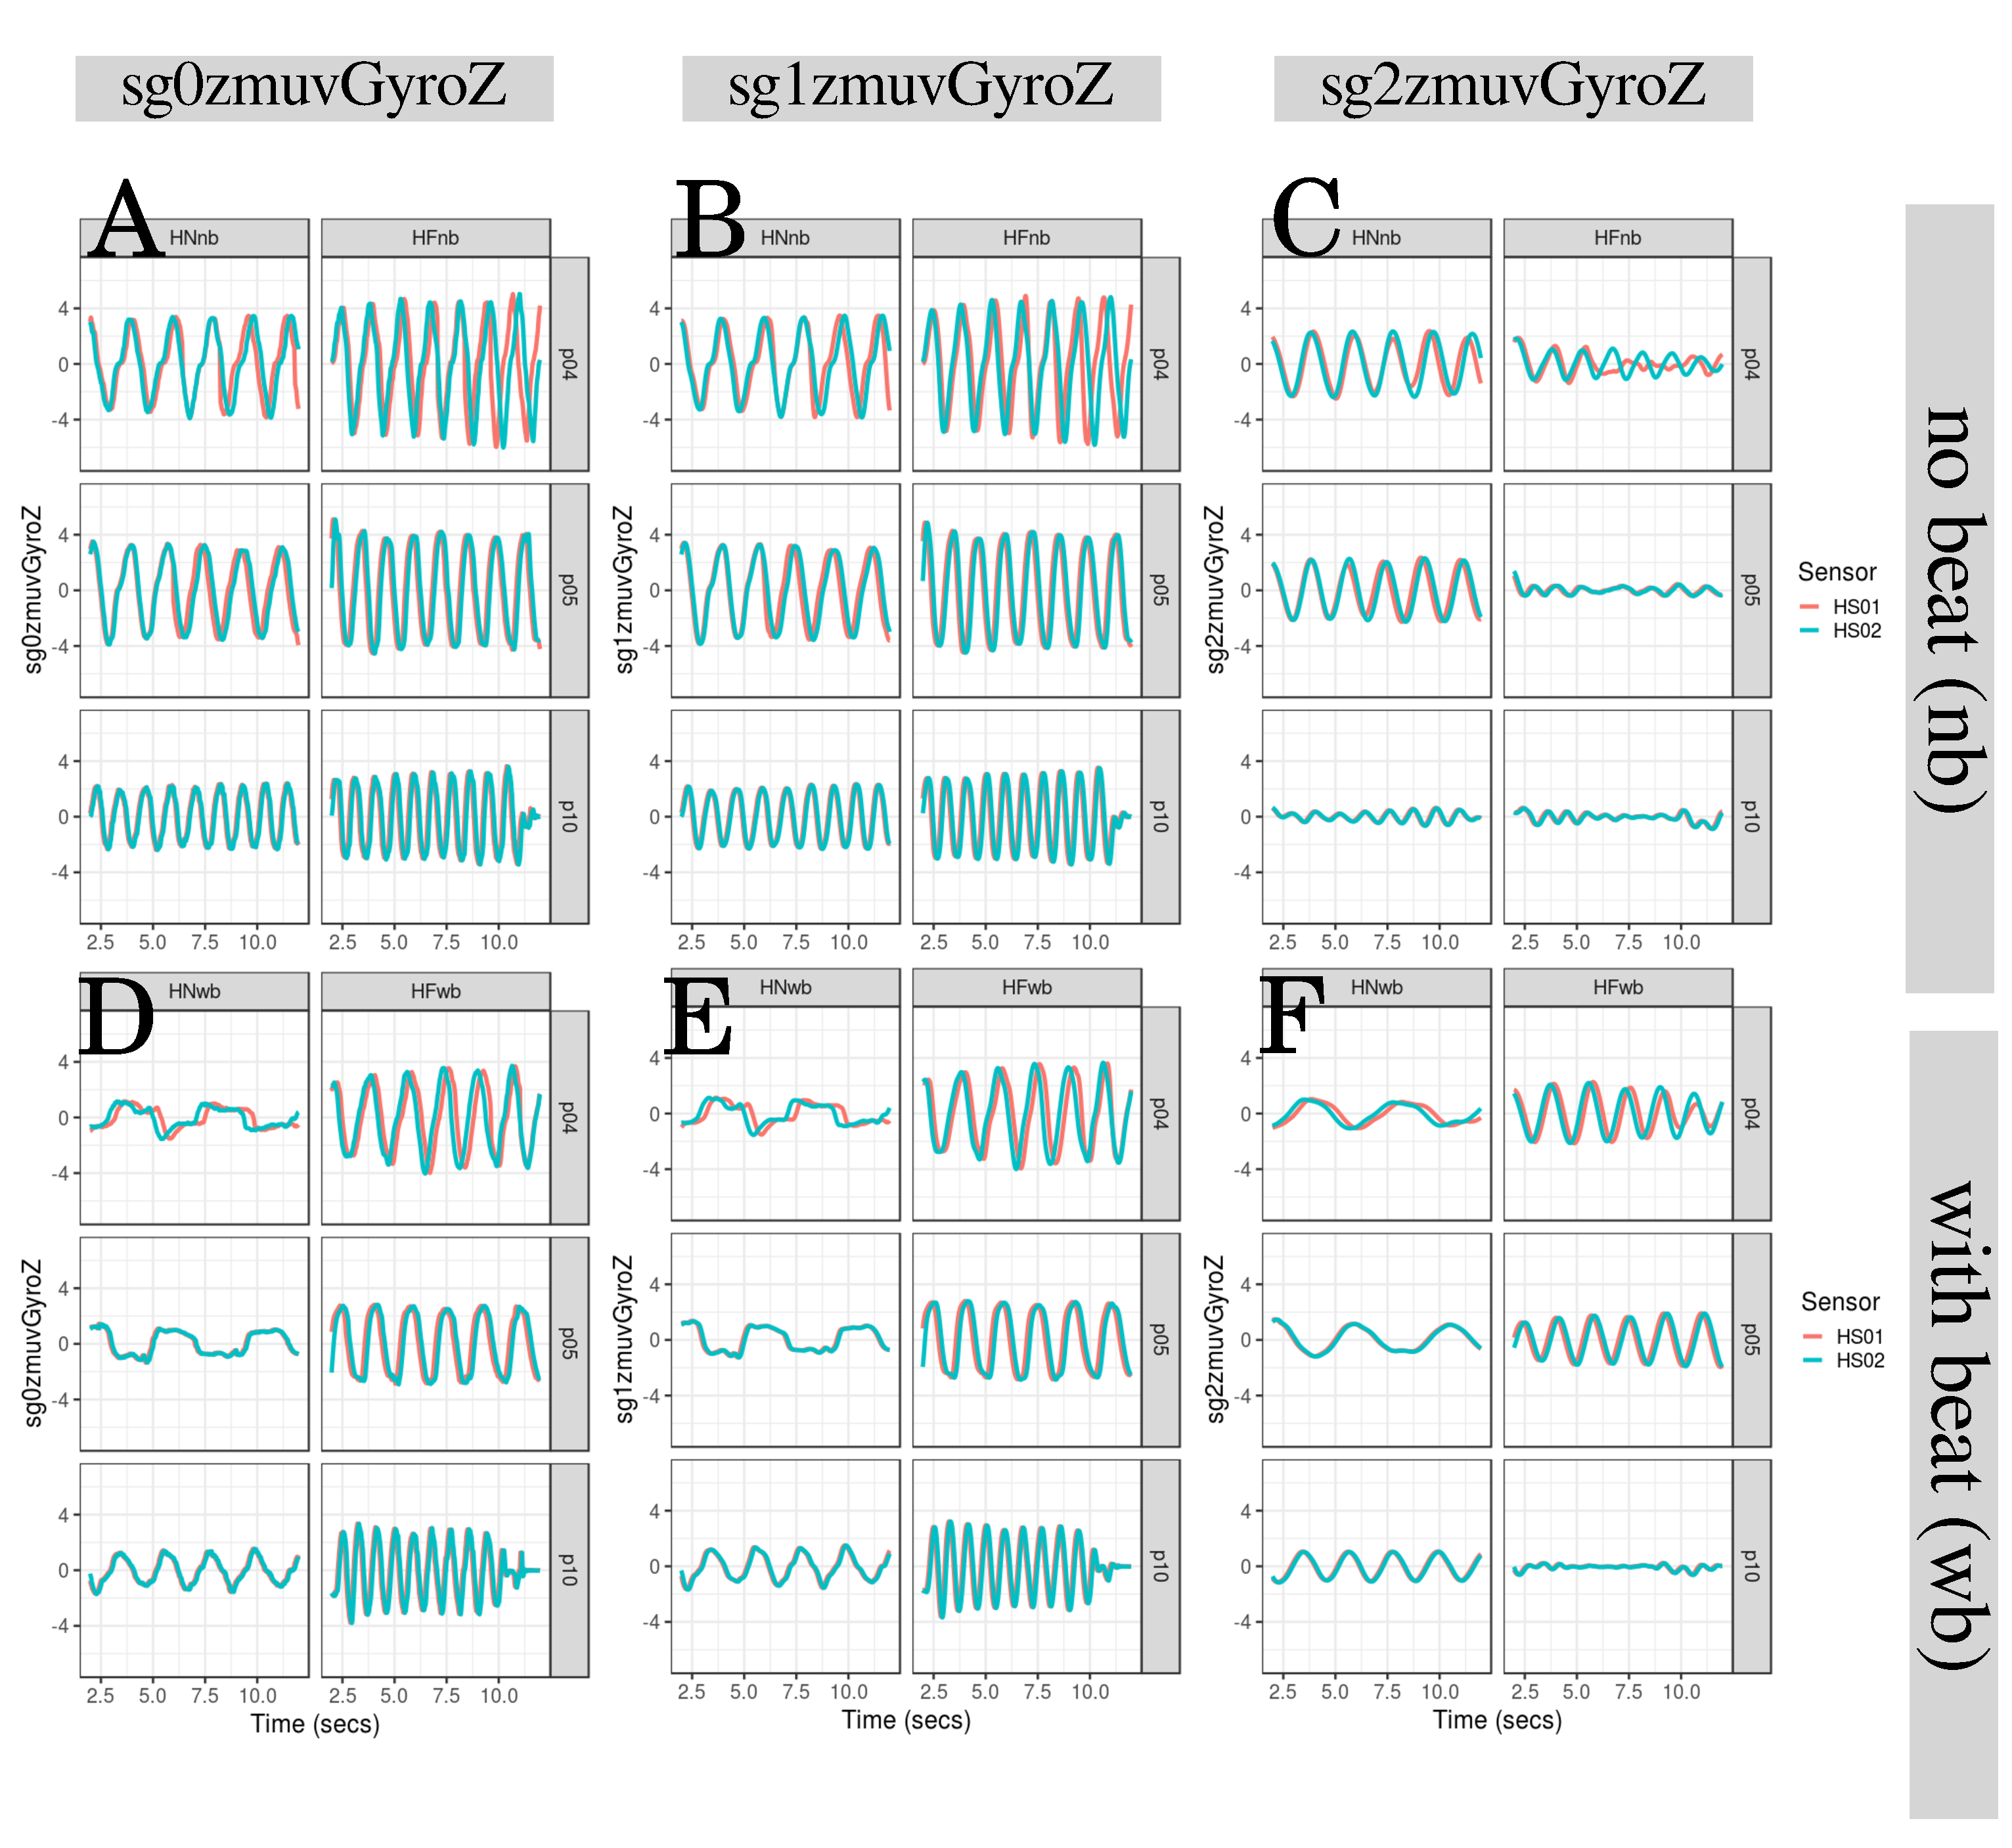
\includegraphics[width=1.0\textwidth]{fig_5_01}
    	\caption
	[Time series for horizontal arm movements]{
	{\bf Time series for horizontal arm movements.}
		Time series for (A,D) raw-normalised (sg0zmuvGyroZ), 
		(B,E) normalised-smoothed 1 (sg1zmuvGyroZ), and
		(C,F) normalised-smoothed 2 (sg2zmuvGyroZ).
		Time series are for three participants 
		($p04$, $p05$, and $p10$) 
		for horizontal movements in normal and faster velocity with
		no beat	(HNnb, HFnb) and with beat (HNwb, HFwb) using 
		the normalised GyroZ axis (zmuvGyroZ) and 
		two sensors attached to the participant wrist (HS01, HS02).
	R code to reproduce the figure is available from \cite{xochicale2018}.
        }
    \label{fig:tsH-hii}
\end{figure}
%%---------------------------------(FIGURE)-----------------------------------
%%---------------------------------(FIGURE)-------------------------------------
\begin{figure}
\centering
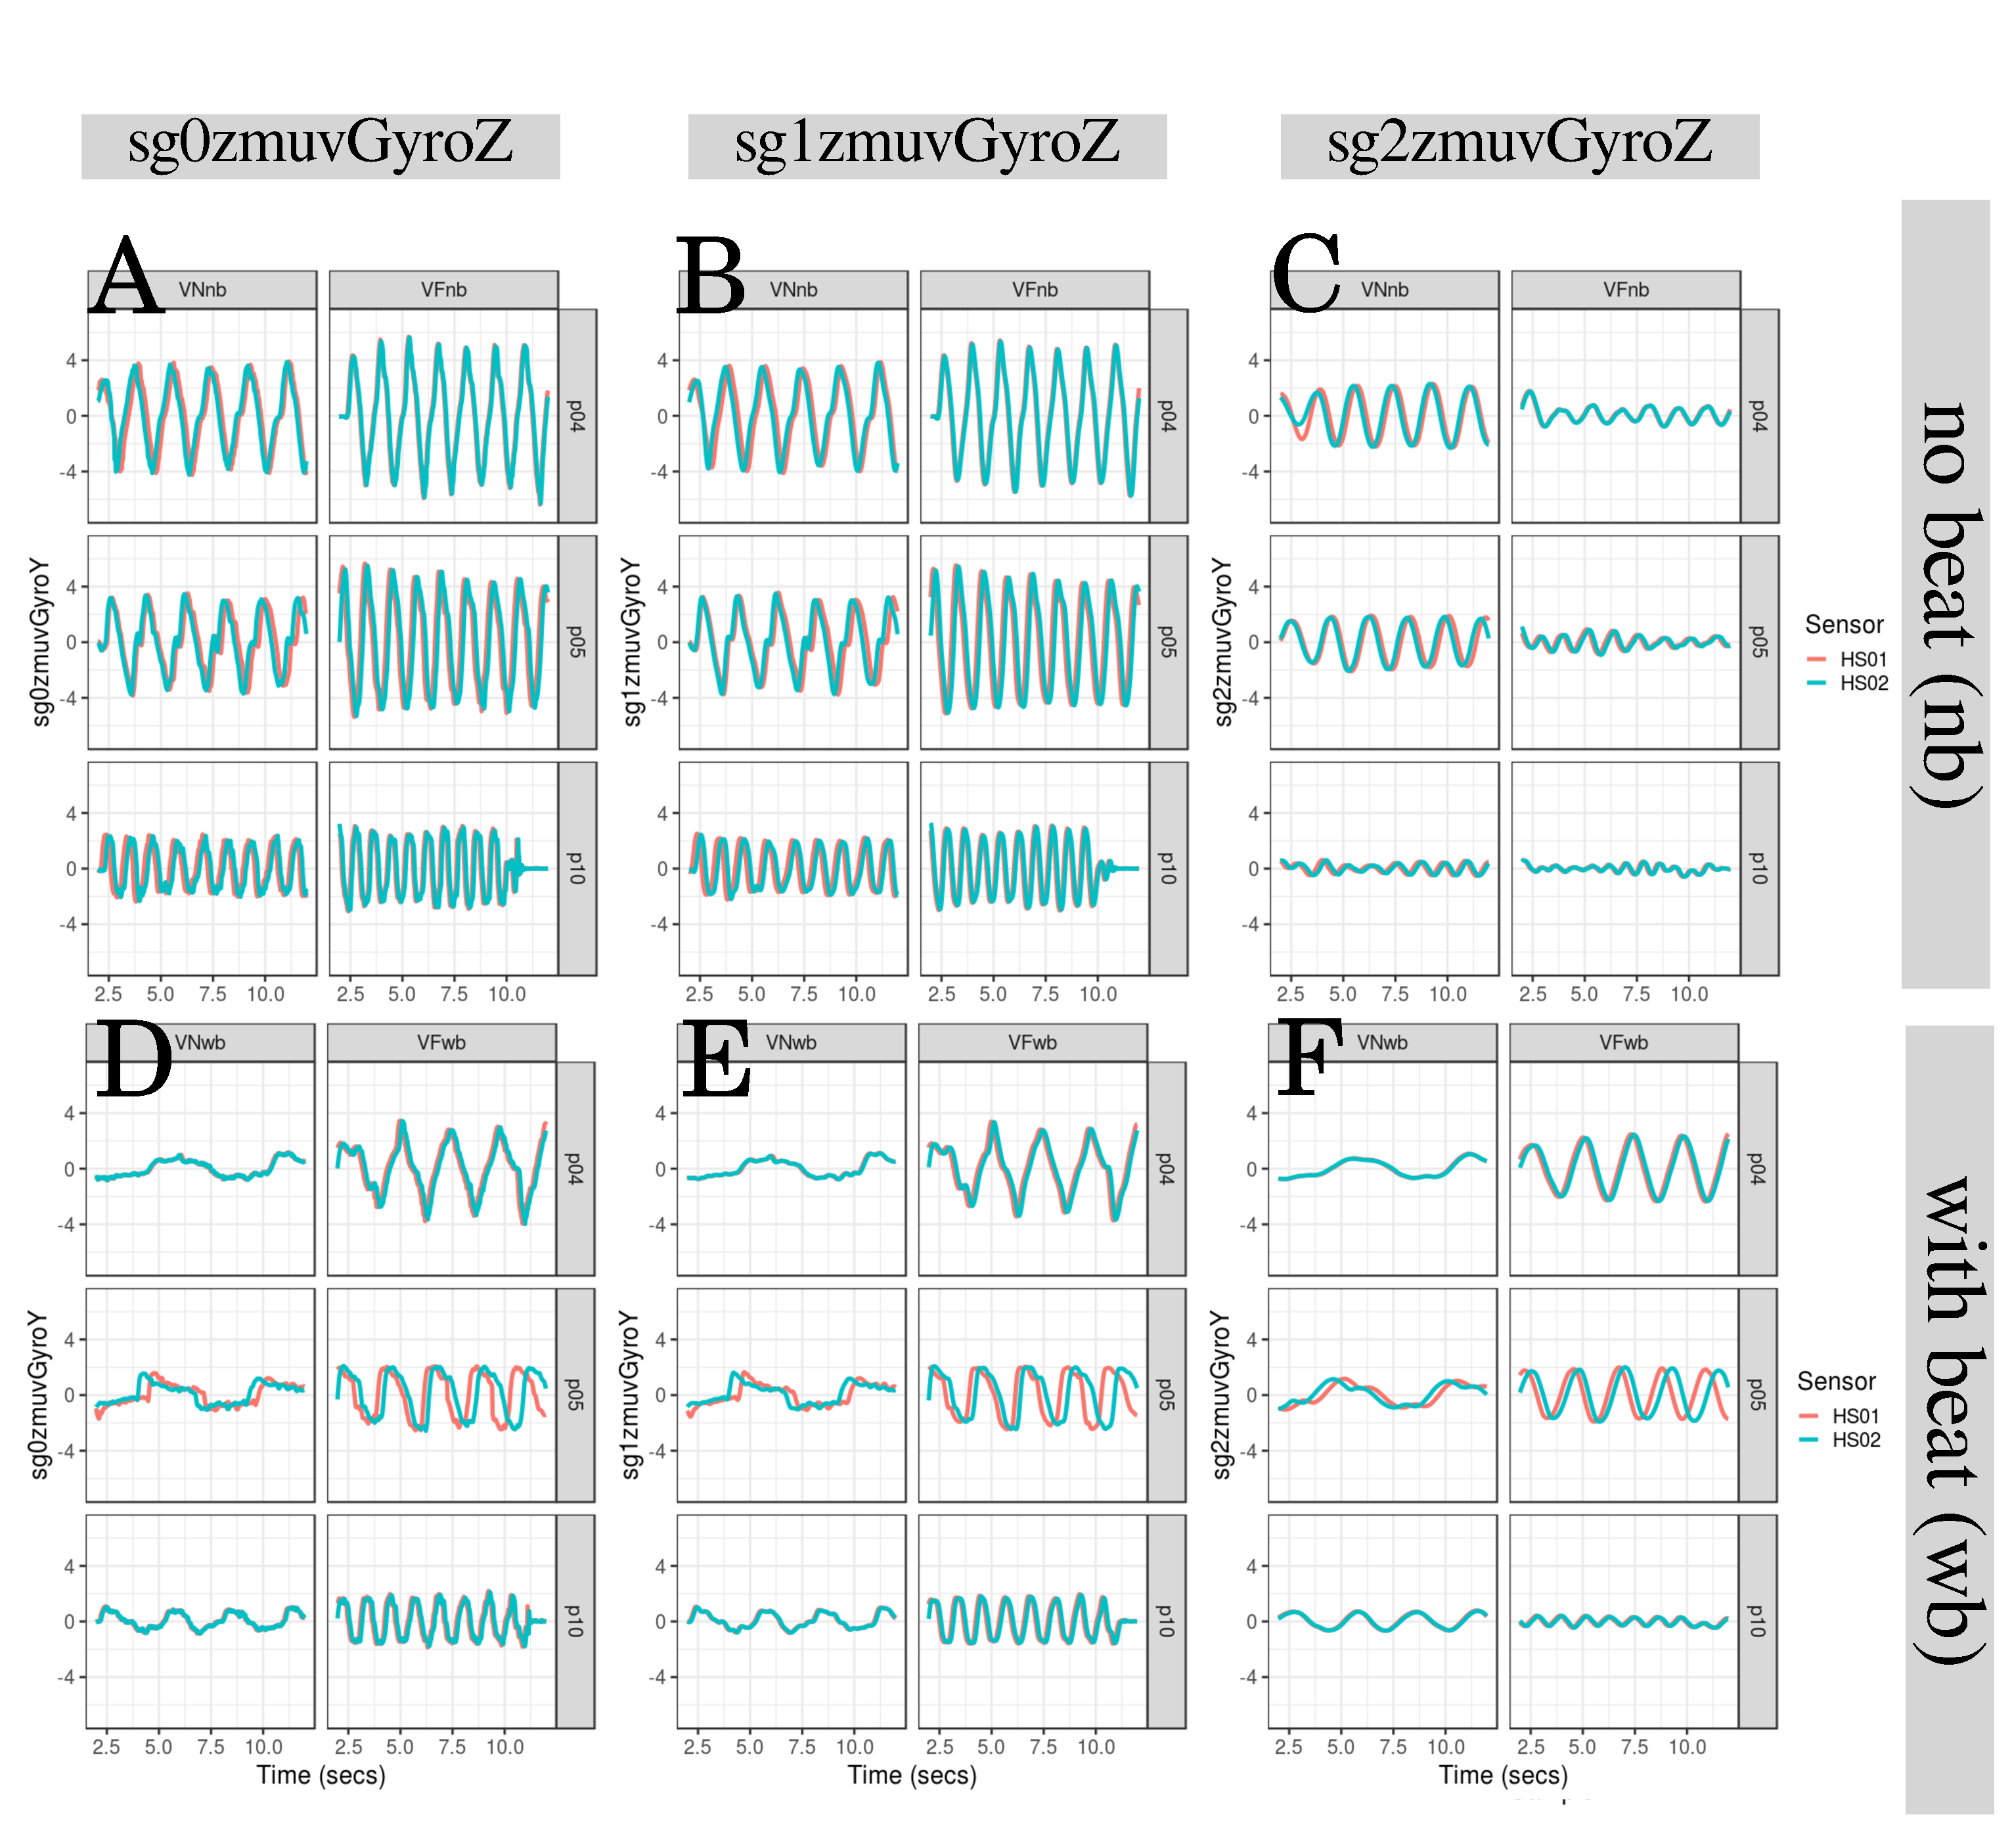
\includegraphics[width=1.0\textwidth]{fig_5_02}
    	\caption
	[Time series for vertical arm movements]{
	{\bf Time series for vertical arm movements.}
		Time series for (A,D) raw-normalised (sg0zmuvGyroY), 
		(B,E) normalised-smoothed 1 (sg1zmuvGyroY), and
		(C,F) normalised-smoothed 2 (sg2zmuvGyroY).
		Time series are for three participants 
		($p04$, $p05$, and $p10$) 
		for vertical movements in normal and faster velocity with
		no beat	(VNnb, VFnb) and with beat (VNwb, VFwb) using the 
		normalised GyroY axis (zmuvGyroY) and two sensors 
		attached to the participant wrist (HS01, HS02).
	R code to reproduce the figure is available from \cite{xochicale2018}.
        }
    \label{fig:tsV-hii}
\end{figure}
%%---------------------------------(FIGURE)------------------------------------

\newpage
\section{Minimum Embedding Parameters} \label{mep-hii}
The first step to create Reconstructed State Spaces (RSSs) with the use of
Uniform Time-Delay Embedding (UTDE) is to compute the
average minimum embedding parameters for all participants, sensors and 
activities using False Nearest Neighbour (FNN) and 
Average Mutual Information (AMI) algorithms.

%\subsection{Minimum dimension embedding values}
Hence, Figs. \ref{fig:CAO-hii} illustrate the box plots for minimum 
embedding dimensions.
For horizontal arm movements (Figs. \ref{fig:CAO-hii}(A)), 
one can notice how the interquartile range  
appear to be near to one independently of the 
activity or sensor. 
With regards to the level of smoothness,
there is a decrease of sample mean (gray rhombus) 
as the smoothness increase.  
Similarly, for vertical arm movements (Figs. \ref{fig:CAO-hii}(B))
the interquartile range of activities and sensors 
appears to be near to one. In addition to that, 
the increase of smoothness is affected by a decrease 
in sample means (gray rhombus) meaning that there is 
a decrease of dimensionality of the dynamics of 
the time series data.
For further details of the minimum dimension values see 
Figs \ref{fig:caoHnb}, \ref{fig:caoHwb}, \ref{fig:caoVnb} and 
\ref{fig:caoVwb} in Appendix \ref{appendix:d:ep}.
%%---------------------------------(FIGURE)-------------------------------------
\begin{figure}
\centering
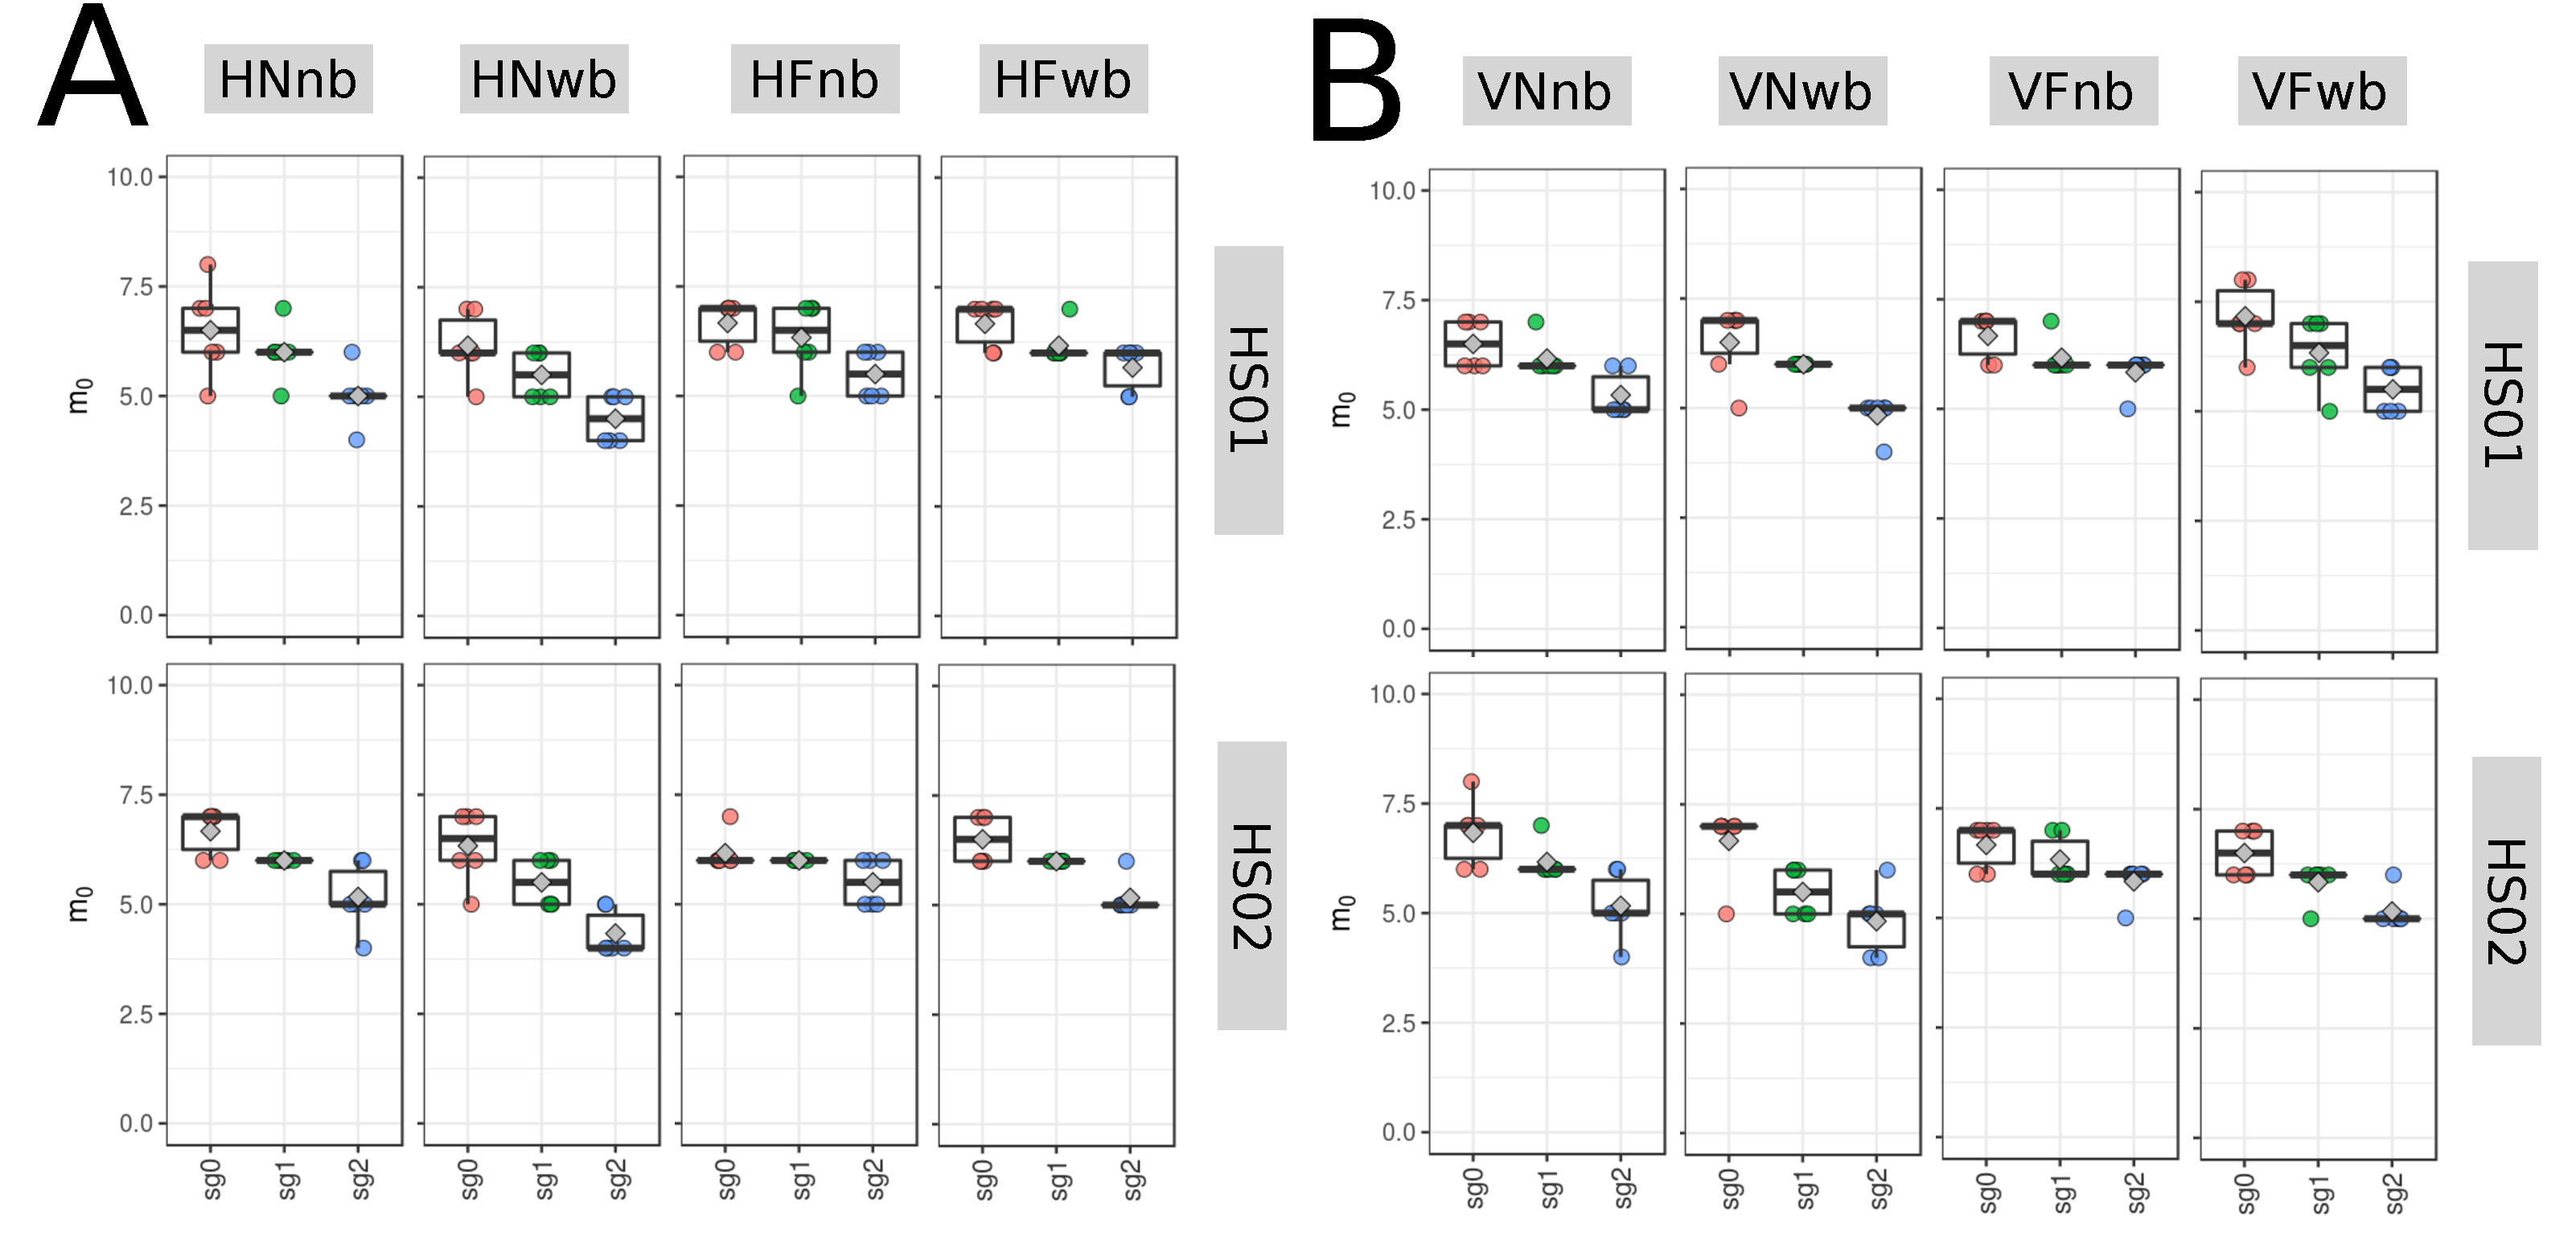
\includegraphics[width=0.95\textwidth]{fig_5_03}
	\caption
	[Box plots for minimum embedding dimensions]{
	{\bf Box plots for minimum embedding dimensions.} 
		Box plots of minimum embedding dimensions for 
		(A) horizontal and (B) vertical arm movements for
		normal  and faster velocity (N/F) with no beat (nb) 
		and with beat (wb) movements
		using sensors 01 and 02 attached to the wrist of the 
		participant (HS01, HS02).
		Minimum embedding dimensions are for six participants 
		($p01$, $p04$, $p05$, $p10$, $p11$, $p15$) with three 
		smoothed signals (sg0, sg1 and sg2)
		and window length of 10-sec (500 samples).
		R code to reproduce the figure is available 
		from \cite{xochicale2018}.
        }
    \label{fig:CAO-hii}
\end{figure}
%%---------------------------------(FIGURE)-------------------------------------

%\subsection{Minimum delay embedding values}
Figs. \ref{fig:AMI-hii} illustrate the box plots for first minimum AMI.
Box plots for horizontal arm movements (Figs. \ref{fig:AMI-hii}(A)) for 
HNwb appear more spread (interquartile range between 10 to 20) while 
other activities there is a slight variation of values 
(interquartile range between 5 to 10).
Little can be said regardless the sample mean of each axis (gray rhombus) 
which is not proportionally affected as the smoothed of the time series 
increase.
Box plots for vertical arm movements (Figs. \ref{fig:AMI-hii}(B)) 
show that the interquartile range of each activity is constant
except for the activity VFwb.
Additionally, the increase of smoothness of time series (sg0 to sg2) made 
the sample mean (gray rhombus) to increase which means that 
the maximal information to knowledge from $x(n)$ to $x(t+\tau_0)$ also 
increase.
For further details of the miminum dimension values see 
Figs \ref{fig:amiHnb}, \ref{fig:amiHwb}, \ref{fig:amiVnb} and \ref{fig:amiVwb}
in Appendix \ref{appendix:d:ep}.
%%---------------------------------(FIGURE)-------------------------------------
\begin{figure}
\centering
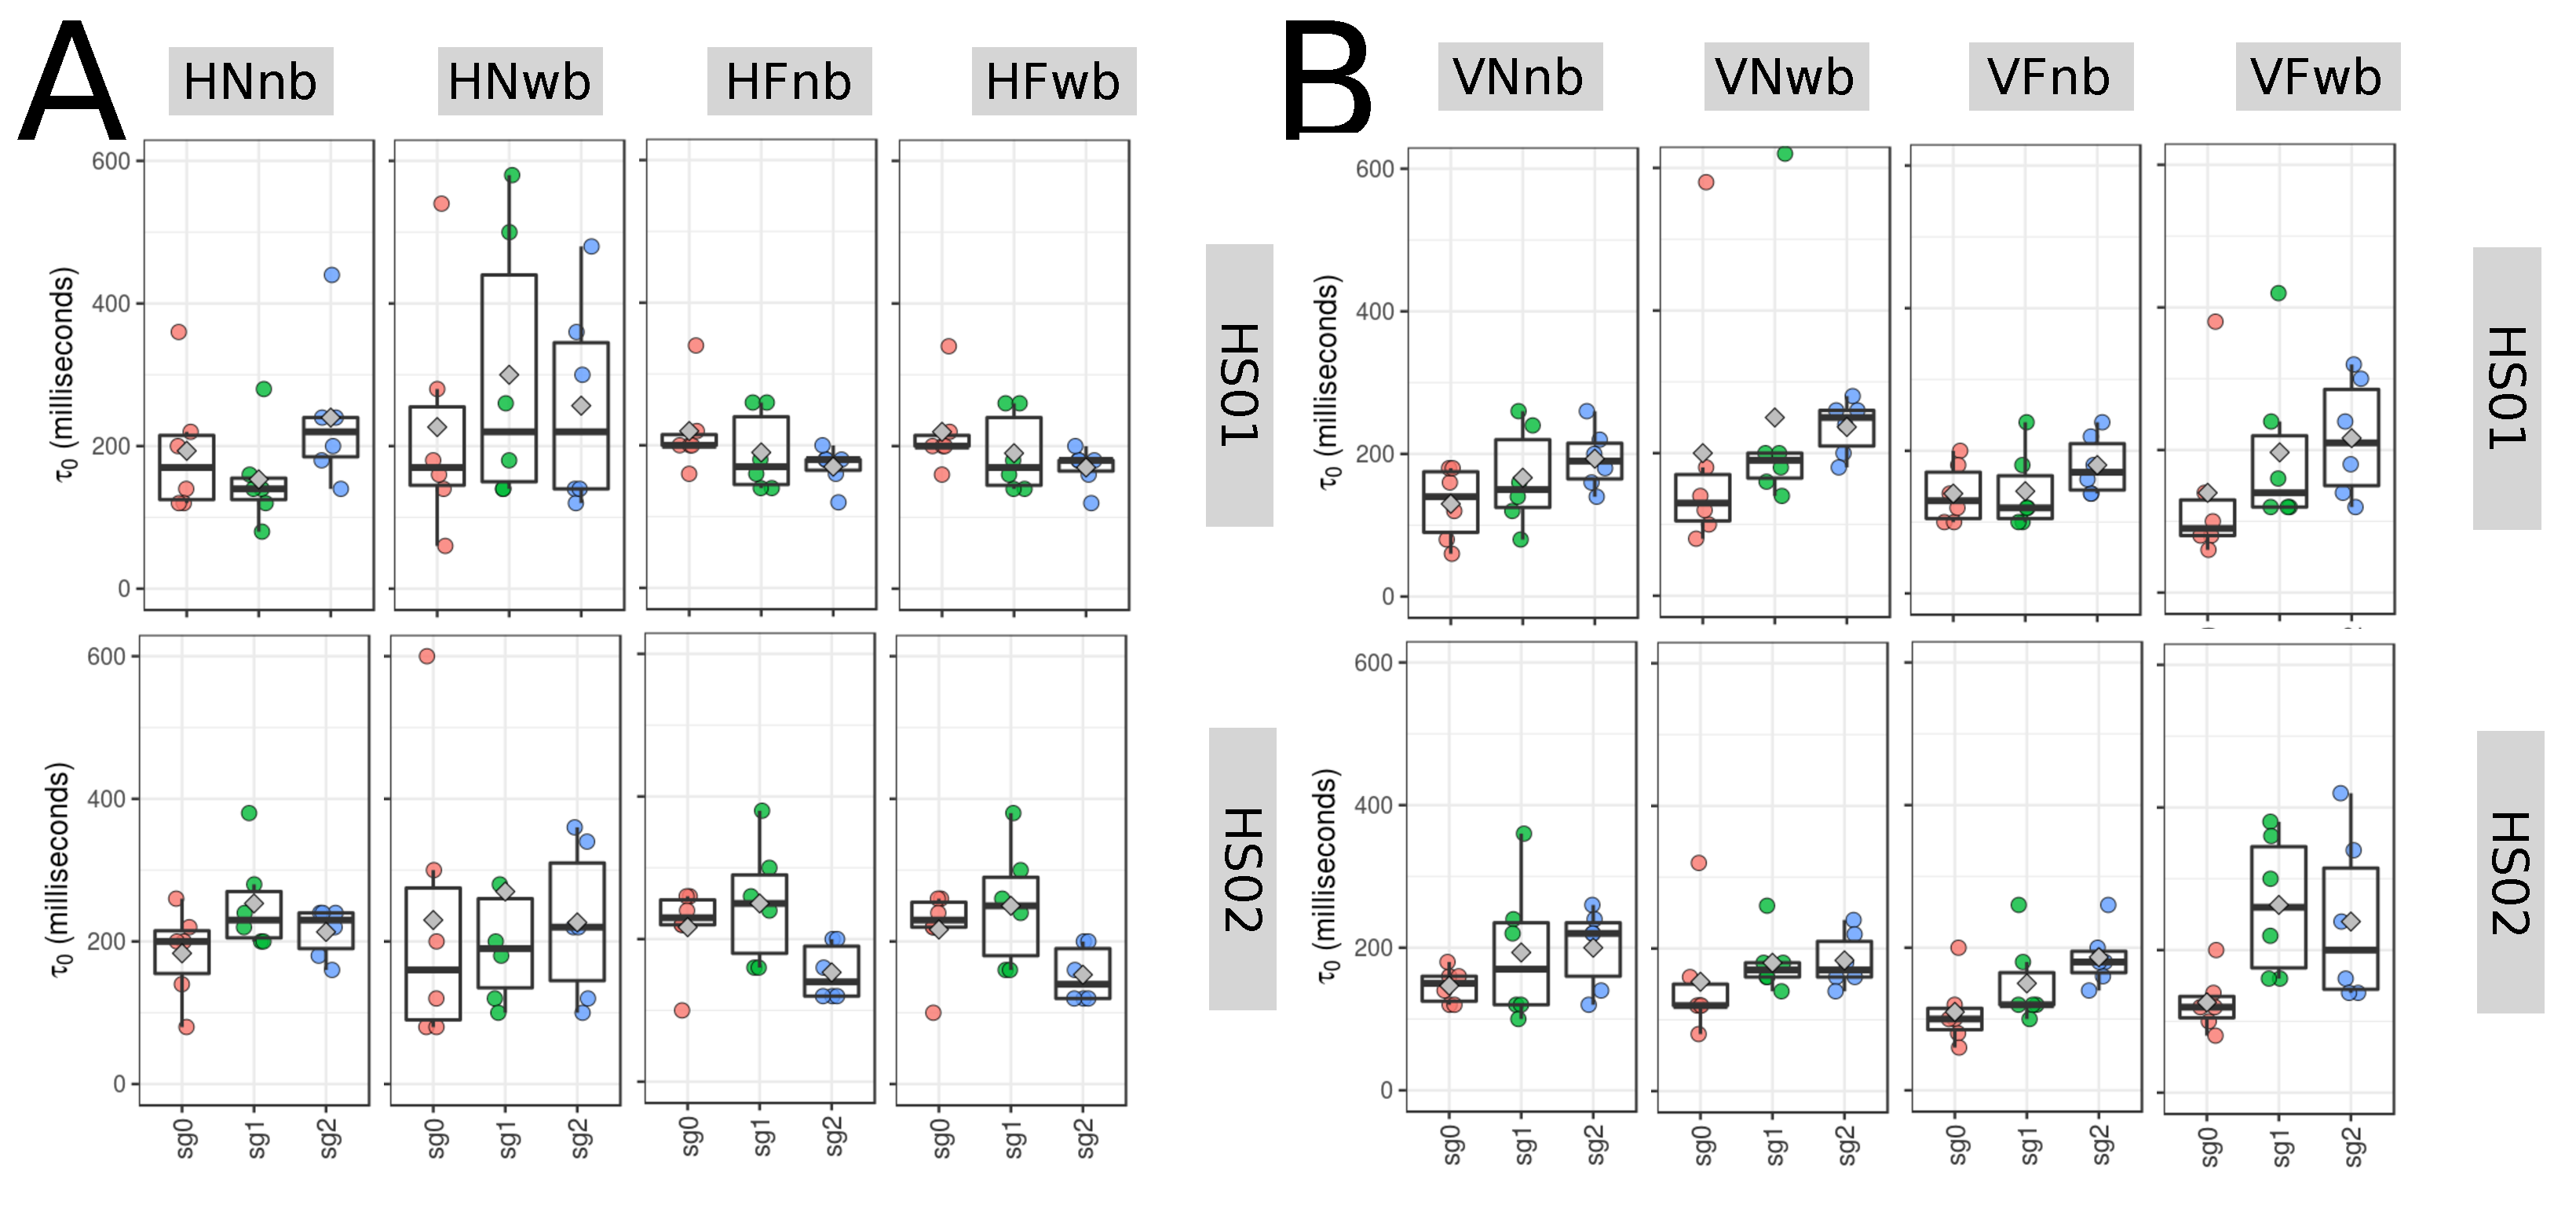
\includegraphics[width=0.95\textwidth]{fig_5_04}
	\caption
	[Box plots for 1st minimum AMI]{
	{\bf Box plots for 1st minimum AMI.} 
		Box plots of the 1st minimum AMI values for 
		(A) horizontal and (B) vertical arm movements for
		normal and faster velocity (N/F) with no beat (nb) 
		and with beat (wb) movements
		using sensors 01 and 02 attached to the wrist of the 
		participant (HS01, HS02).
		First minimum AMI values in milliseconds are 
		for six participants 
		($p01$, $p04$, $p05$, $p10$, $p11$, $p15$) with three 
		smoothed signals (sg0, sg1 and sg2)
		and window lenght of 10-sec (500 samples).
		R code to reproduce the figure is available 
		from \cite{xochicale2018}.
        }
    \label{fig:AMI-hii}
\end{figure}
%%---------------------------------(FIGURE)-------------------------------------

\newpage
\subsection{Average minimum embedding parameters}
Although the implementation of Uniform Time-Delay Embedding (UTDE) 
is simple, the main challenge is the selection of appropriate embedding 
parameters to reconstruct the state spaces of each time series
as these are unique in terms of its structure (modulation of amplitude, 
frequency and phase) \citep{ frank2010, sama2013, bradley2015}.
With that in mind, one problem we faced in this thesis is the
selection of embedded parameters that can represent all time series. 
The solution to that problem was to compute a sample mean over 
all values for all participants, activities and sensors
(Section \ref{sec:overall_minMT}).
Hence, the average minimum embedding parameters is computed with 
a sample mean of $\overline{m}_0=6$ from the minimum values 
of $E_{1}(m)$ in Figs \ref{fig:CAO-hii} and a sample mean 
of $\overline{\tau}_0=10$ from minimum values of AMIs in Figs \ref{fig:AMI-hii}.
Hence, Reconstructed State Spaces (RSSs), Recurrence Plots (RPs) and
Recurrence Quantification Analysis (RQA) metrics
are computed with the average minimum embedding parameters 
($\overline{m_0}=6$, $\overline{\tau_0}=10$).

\section{Reconstructed state spaces with UTDE}
Reconstructed state spaces for horizontal normal and horizontal faster 
arm movements with no beat are shown in Fig \ref{fig:rss_Hnb_w500}.
The smoothness of the time series show a slightly change of smoothed 
trajectories in the RSSs for sg0zmuvGyroZ and sg1zmuvGyroZ, while the 
RSSs trajectories for sg2zmuvGyroZ appear to be distorted 
(Fig \ref{fig:rss_Hnb_w500}).
One can see slightly differences in the RSSs trajectories when comparing 
sensors HS01 and HS02 for horizontal normal arm movement with no beat 
(Fig \ref{fig:rss_Hnb_w500}(A, B)) and horizontal faster arm movements 
with no beat (Fig \ref{fig:rss_Hnb_w500}(C, D)).
With regards to the type of movement, the RSSs trajectories appear 
to change little when comparing horizontal normal with faster arm movements 
(Fig \ref{fig:rss_Hnb_w500}).

Fig \ref{fig:rss_Hwb_w500} shows trajectories of the reconstructed 
state space for horizontal normal and horizontal faster arm movements 
while beat sounds. Hence, as in Fig \ref{fig:rss_Hnb_w500}, 
it can also be noted in Fig \ref{fig:rss_Hwb_w500} that the smoothness 
of sg0zmuvGyroZ and sg1zmuvGyroZ appear to affect little the RSSs 
trajectories, while RSSs trajectories for sg2zmuvGyroZ substantially change 
so as to show different patterns. However, the trajectories in the RSS 
appear to change little when comparing the differences between the type 
of sensors HS01 and HS02 (Fig \ref{fig:rss_Hwb_w500}).
For the type of movements, trajectories show differences for horizontal
normal and horizontal faster arm movements (Fig \ref{fig:rss_Hwb_w500}).

Fig \ref{fig:rss_Vnb_w500} show trajectories for reconstructed state spaces
of vertical normal and vertical faster arm movements with no beat. 
Smoothness of the RSSs trajectories is slightly noticed for sg0zmuvGyroY and
sg1zmuvGyroY, whereas RSSs trajectories for sg2zmuvGyroY are evidently 
different (Fig \ref{fig:rss_Vnb_w500}).
When comparing the RSSs trajectories from sensors HS01 and HS02,
it can be noted little change, whereas the comparison from type of movement, 
the trajectories difference is more notable (Fig \ref{fig:rss_Vnb_w500}).

Fig \ref{fig:rss_Vwb_w500} show trajectories for reconstructed state space
of vertical normal and vertical faster arm movements for participants 
hearing a beat. Smoothness of RSSs trajectories appear to show slightly 
differences between sg0zmuvGyroY and sg1zmuvGyroY, however RSSs trajectories 
for sg2zmuvGyroY are different (Fig \ref{fig:rss_Vwb_w500}).
With regards to the type of sensor HS01 and HS02, RSSs trajectories appear 
to change little, whereas for type of activity of normal and faster arm 
movements, RSSs trajectories show evidently differences 
(Fig \ref{fig:rss_Vwb_w500}).

%%---------------------------------(FIGURE)-------------------------------------
\begin{figure}
\centering
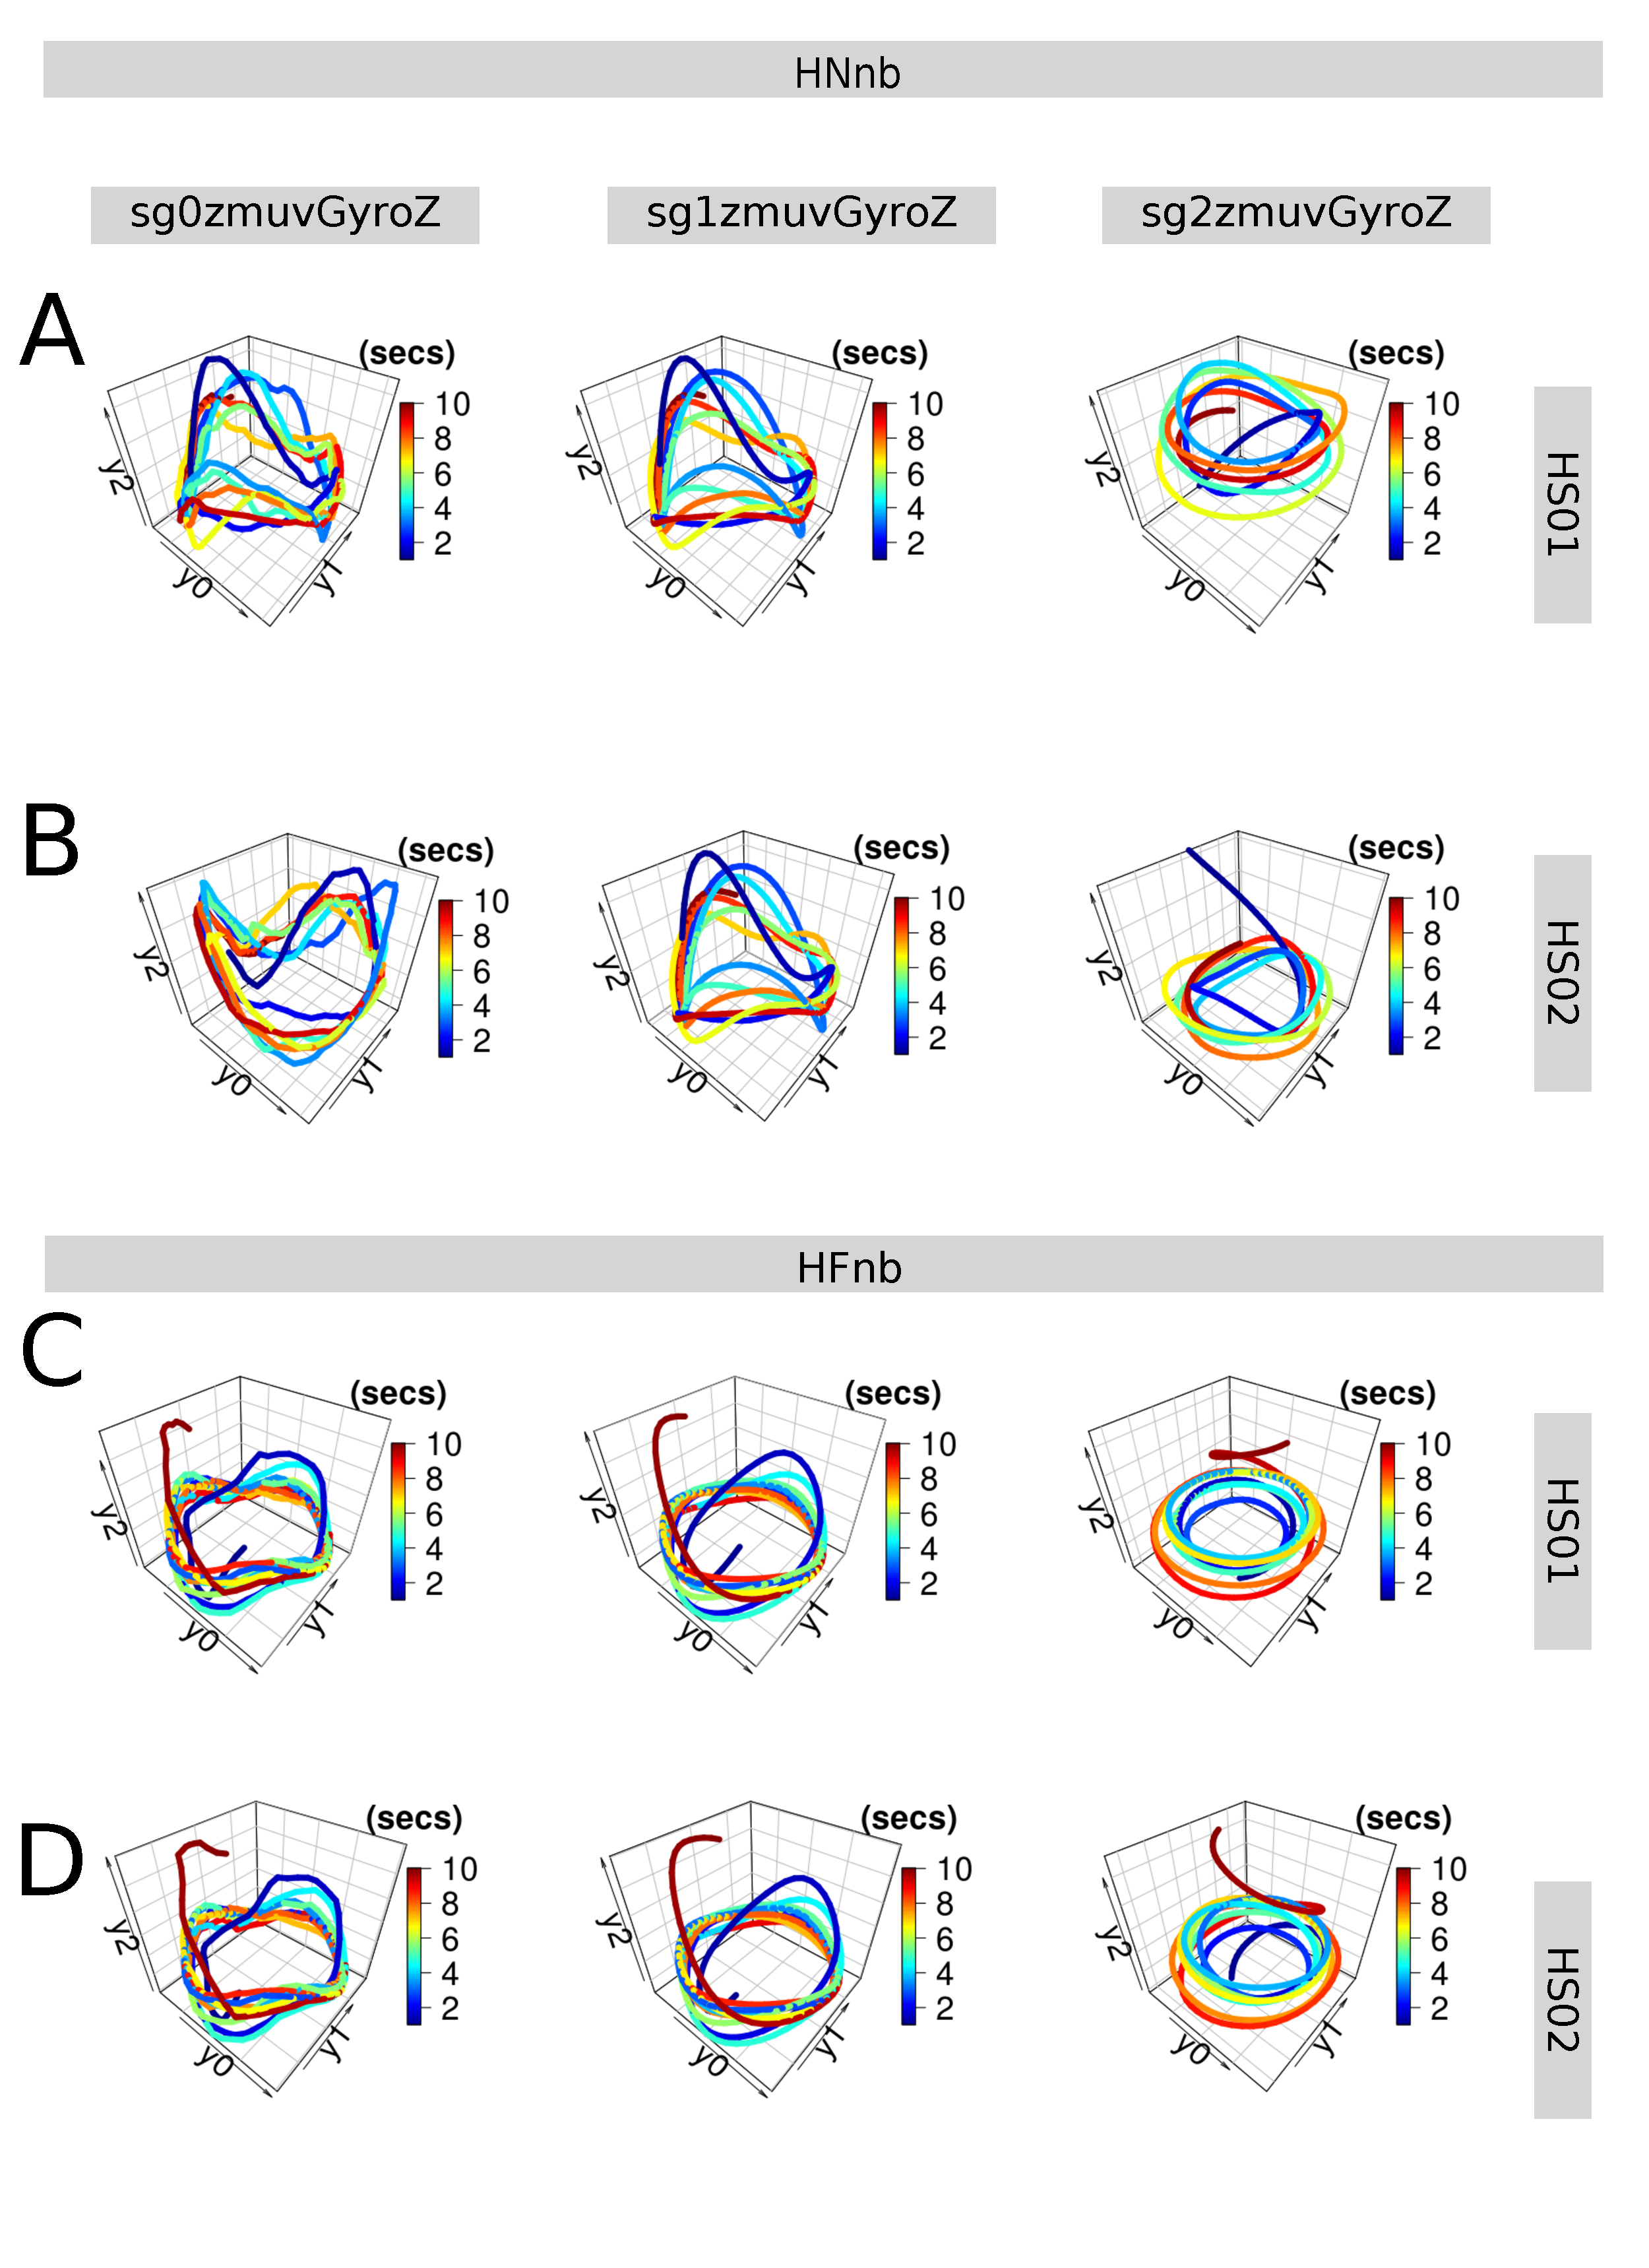
\includegraphics[height=0.8\textheight]{fig_5_05}
\caption
	[RSSs for horizontal arm movements (no beat)]{
	{\bf RSSs for horizontal arm movements (no beat).}
	Reconstructed state spaces of participant p01 for 
	(A, B) horizontal normal movements with no beat (HNnb) and 
	(C, D) horizontal faster velocity with no beat (HFnb).
	Time series for raw-normalised (sg0zmuvGyroZ), 
	normalised-smoothed 1 (sg1zmuvGyroZ) and 
	normalised-smoothed 2 (sg2zmuvGyroZ) with
	(A, C) sensor attached to the participant (HS01), and
	(B, D) sensor attached to the participant (HS02).	
	Reconstructed state spaces were computed with 
	embedding parameters $\overline{m_0}=6$, $\overline{\tau_0}=10$.
	R code to reproduce the figure is available from \cite{xochicale2018}.
        }
     \label{fig:rss_Hnb_w500}
\end{figure}
%%---------------------------------(FIGURE)------------------------------------

%%---------------------------------(FIGURE)-------------------------------------
\begin{figure}
\centering
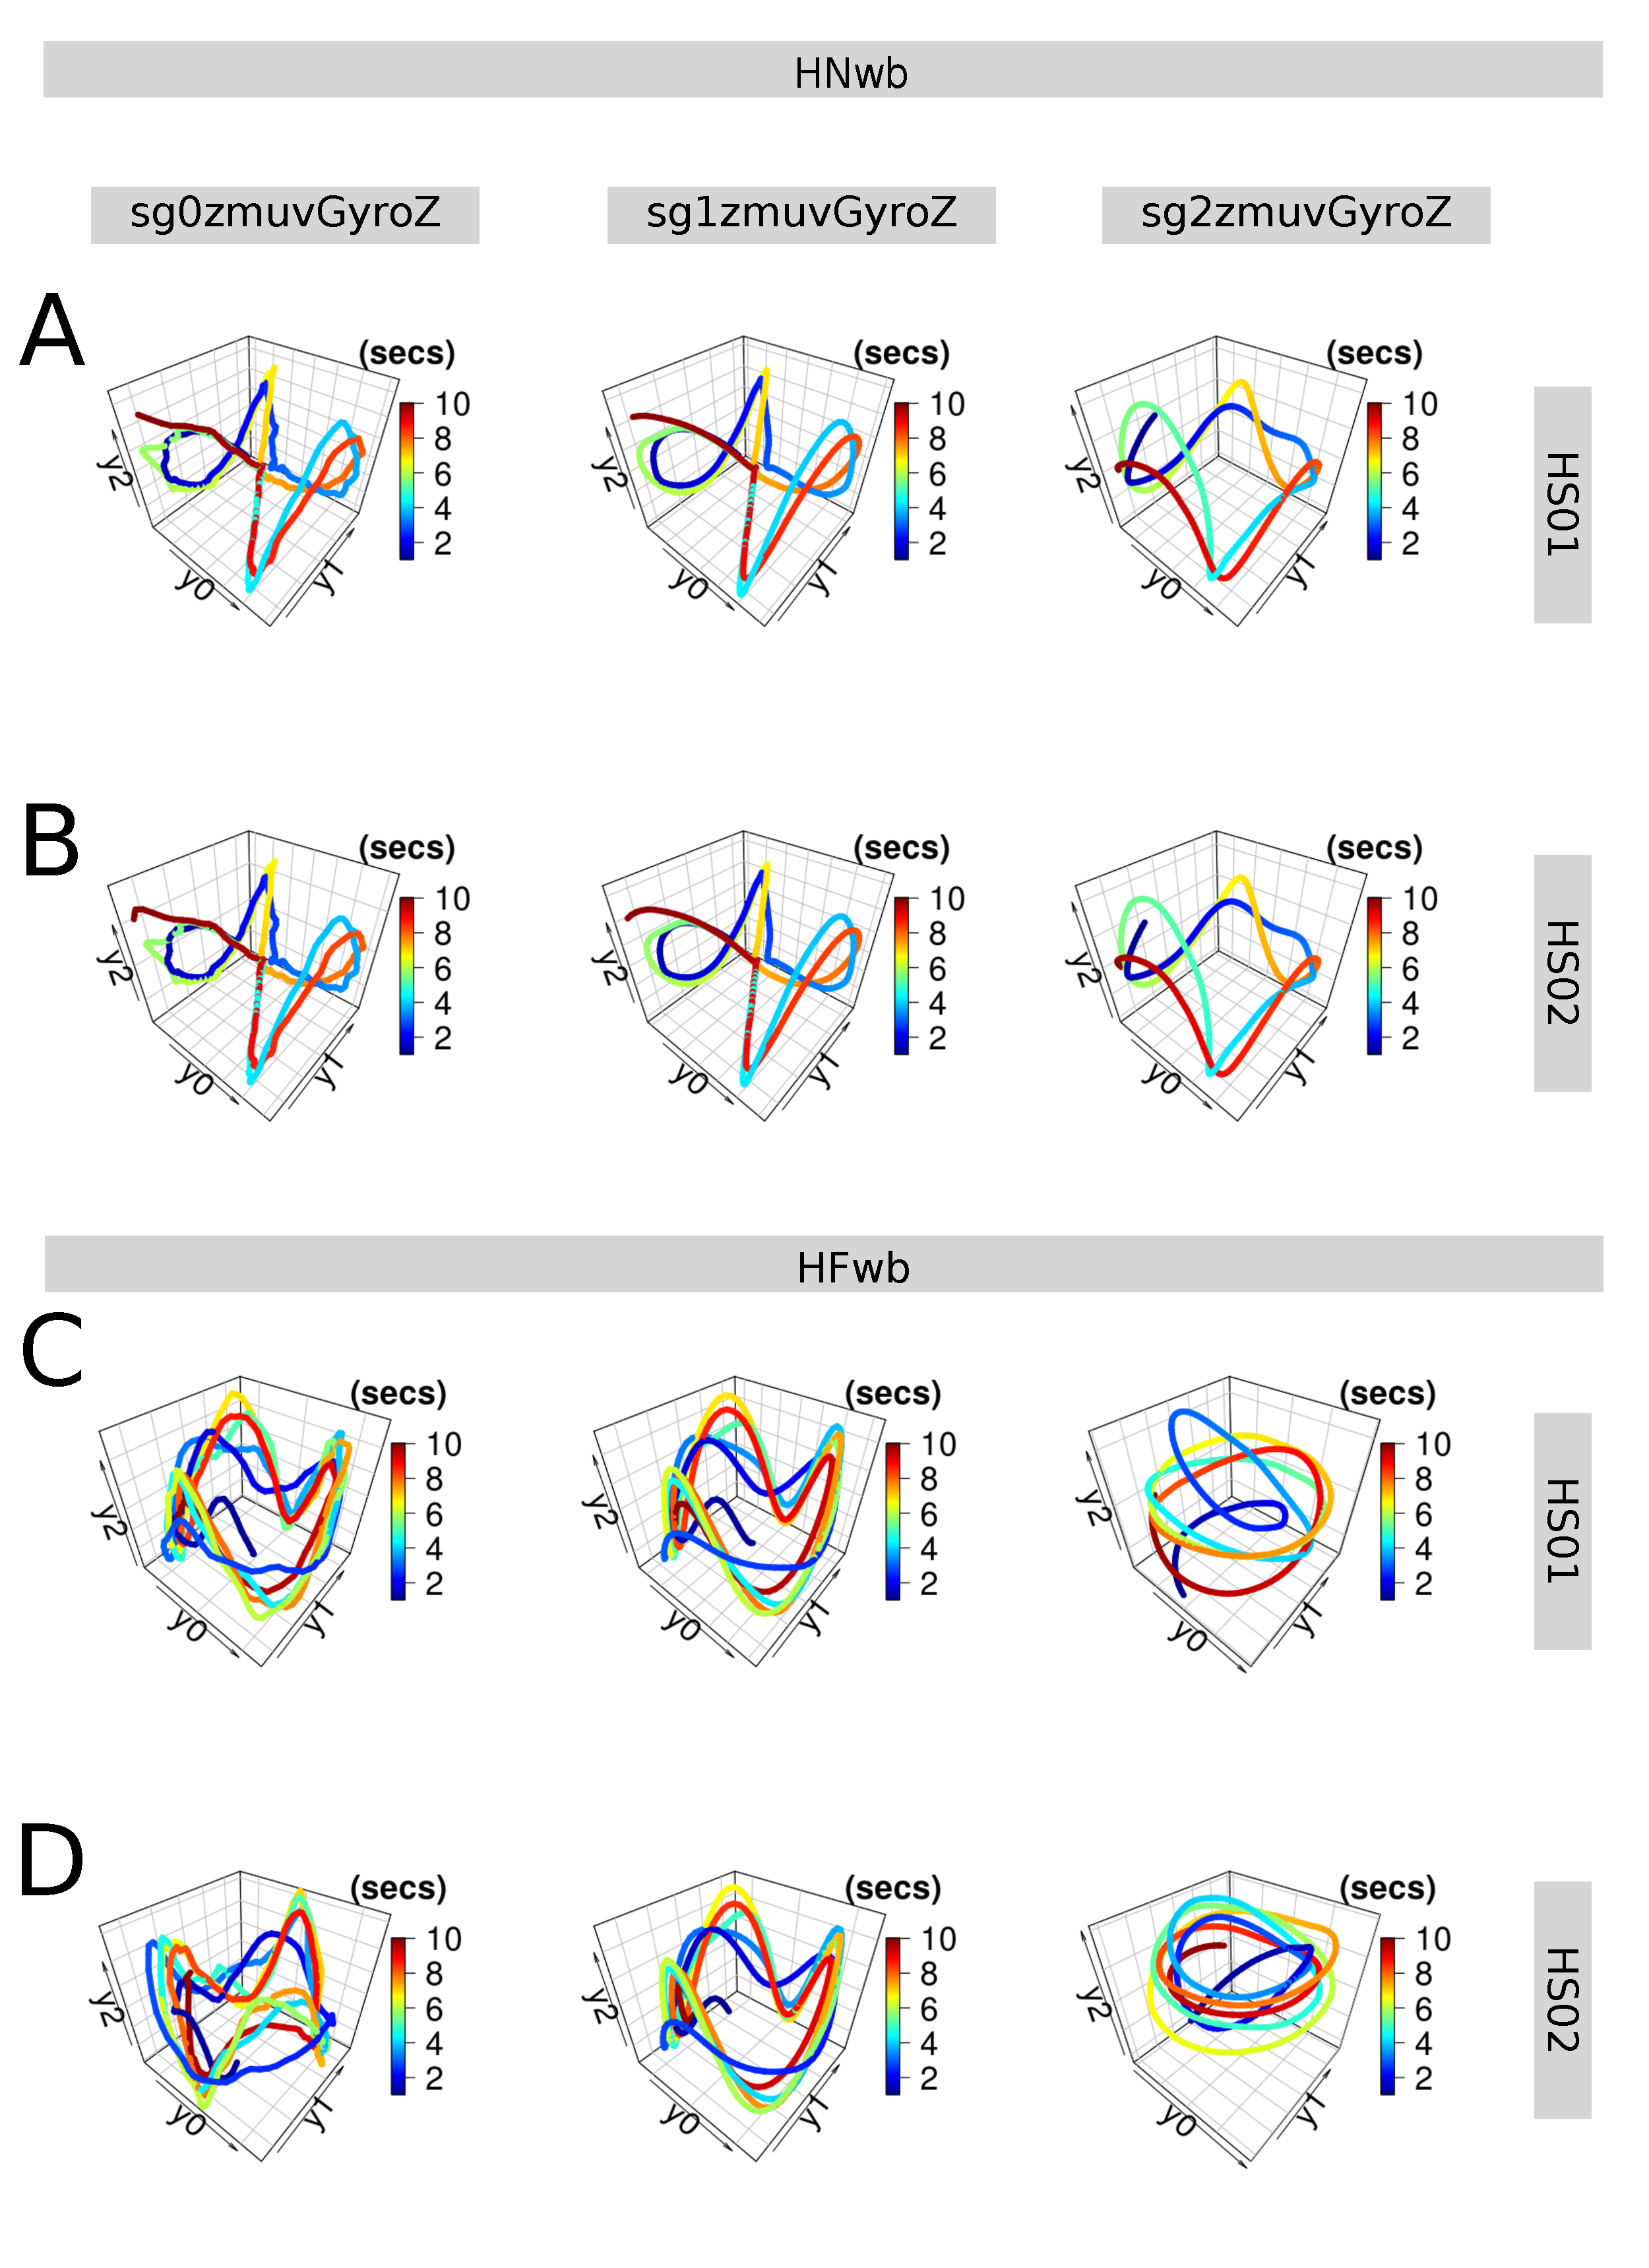
\includegraphics[height=0.8\textheight]{fig_5_06}
\caption
	[RSSs for horizontal arm movements (with beat)]{
	{\bf RSSs for horizontal arm movements (with beat).}
	Reconstructed state spaces of participant p01 for 
	(A, B) horizontal normal movements with beat (HNwb) and 
	(C, D) horizontal faster velocity with beat (HFwb).
	Time series for raw-normalised (sg0zmuvGyroZ), 
	normalised-smoothed 1 (sg1zmuvGyroZ) and 
	normalised-smoothed 2 (sg2zmuvGyroZ) with
	(A, C) sensor attached to the participant (HS01), and
	(B, D) sensor attached to the participant (HS02).	
	Reconstructed state spaces were computed with 
	embedding parameters $\overline{m_0}=6$, $\overline{\tau_0}=10$.
	R code to reproduce the figure is available from \cite{xochicale2018}.
        }
     \label{fig:rss_Hwb_w500}
\end{figure}
%%---------------------------------(FIGURE)------------------------------------

%%---------------------------------(FIGURE)-------------------------------------
\begin{figure}
\centering
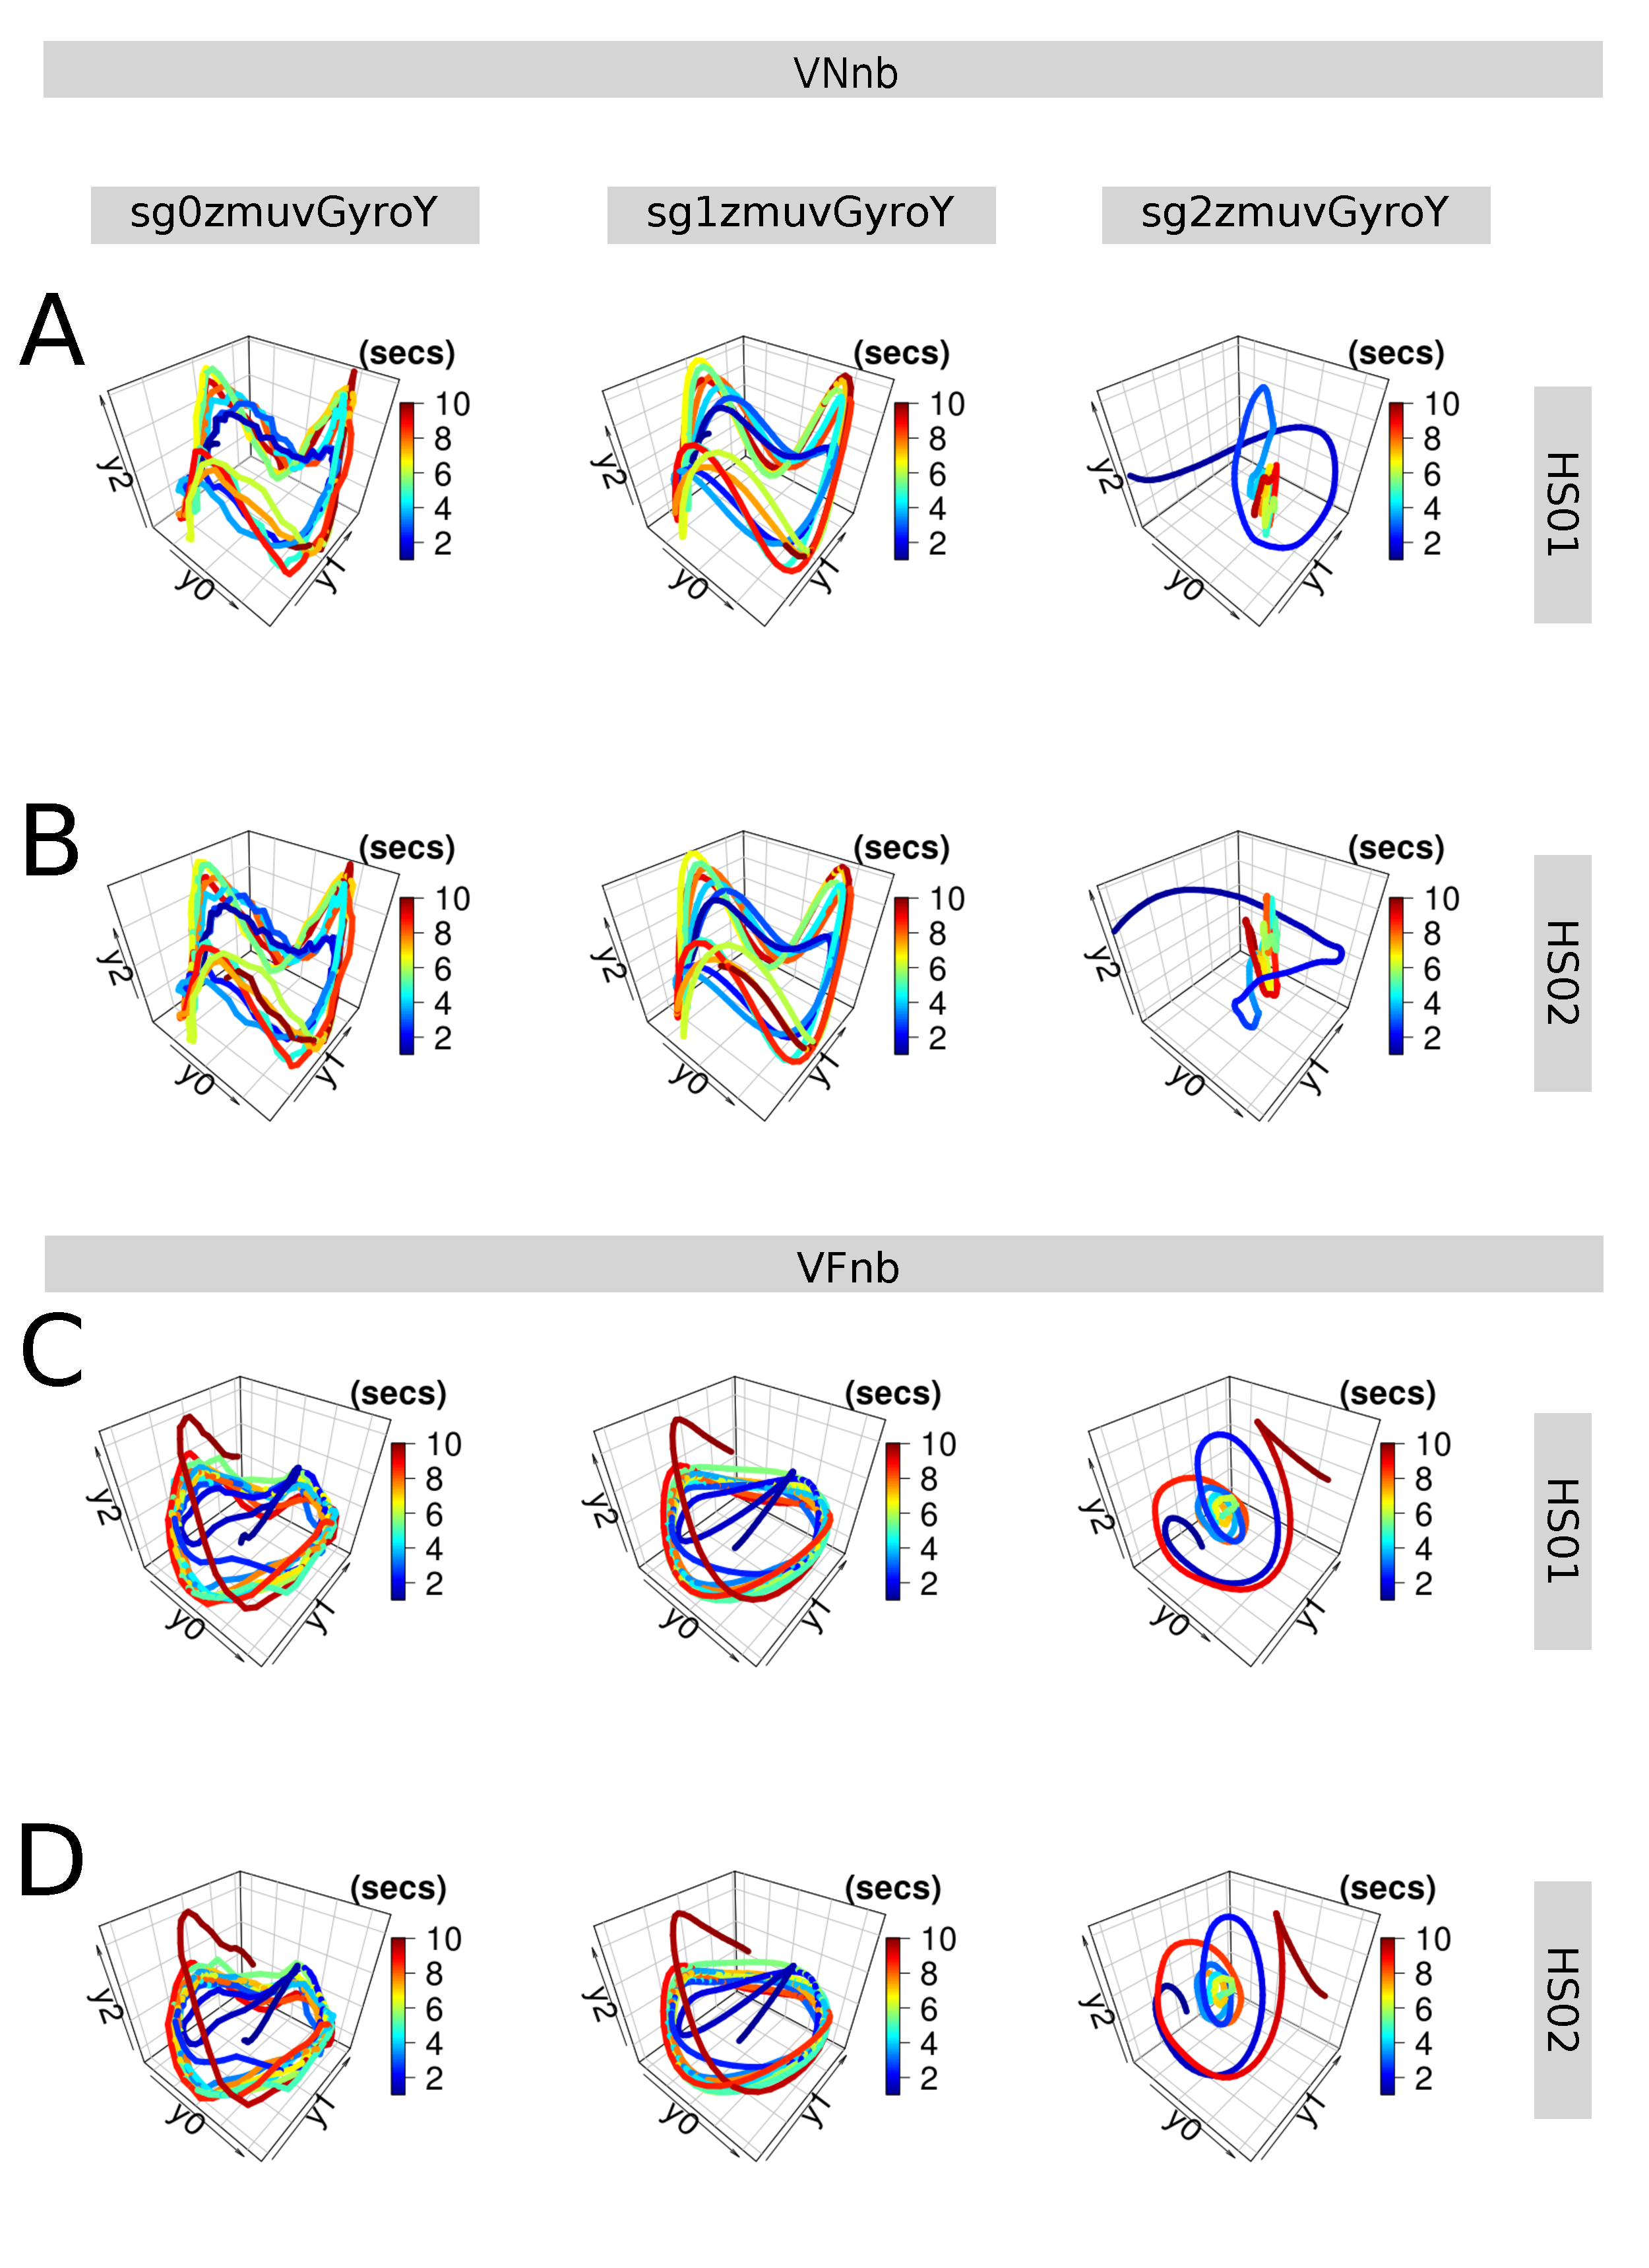
\includegraphics[height=0.8\textheight]{fig_5_07}
\caption
	[RSSs for vertical arm movements (no beat)]{
	{\bf RSSs for vertical arm movements (no beat).}
	Reconstructed state spaces of participant p01 for 
	(A, B) vertical normal movements with no beat (VNnb) and 
	(C, D) vertical faster velocity with no beat (VFnb).
	Time series for raw-normalised (sg0zmuvGyroY), 
	normalised-smoothed 1 (sg1zmuvGyroY) and 
	normalised-smoothed 2 (sg2zmuvGyroY) with
	(A, C) sensor attached to the participant (HS01), and
	(B, D) sensor attached to the participant (HS02).	
	Reconstructed state spaces were computed with 
	embedding parameters $\overline{m_0}=6$, $\overline{\tau_0}=10$.
	R code to reproduce the figure is available from \cite{xochicale2018}.
        }
     \label{fig:rss_Vnb_w500}
\end{figure}
%%---------------------------------(FIGURE)------------------------------------

%%---------------------------------(FIGURE)-------------------------------------
\begin{figure}
\centering
\includegraphics[height=0.8\textheight]{fig_5_08}
\caption
	[RSSs for vertical arm movements (with beat)]{
	{\bf RSSs for vertical arm movements (with beat).}
	Reconstructed state spaces of participant p01 for 
	(A, B) vertical normal movements with beat (VNwb) and 
	(C, D) vertical faster velocity with beat (VFwb).
	Time series for raw-normalised (sg0zmuvGyroY), 
	normalised-smoothed 1 (sg1zmuvGyroY) and 
	normalised-smoothed 2 (sg2zmuvGyroY) with
	(A, C) sensor attached to the participant (HS01), and
	(B, D) sensor attached to the participant (HS02).	
	Reconstructed state spaces were computed with 
	embedding parameters $\overline{m_0}=6$, $\overline{\tau_0}=10$.
	R code to reproduce the figure is available from \cite{xochicale2018}.
        }
     \label{fig:rss_Vwb_w500}
\end{figure}
%%---------------------------------(FIGURE)------------------------------------

\newpage
\section{Recurrences Plots}
Patterns of recurrence plots (RPs) are described in this section.
Recurrence plots are computed with embedding parameters 
$\overline{m_0}=6$, $\overline{\tau_0}=10$ and a recurrence 
threshold $\epsilon=1$ for participant $p01$ performing horizontal 
and vertical arm movements in normal and faster velocity 
with beat and no beat sound (Figs \ref{fig:rps_Hnb_w500}, 
\ref{fig:rps_Hwb_w500}, \ref{fig:rps_Vnb_w500} and \ref{fig:rps_Vwb_w500}).

Figs \ref{fig:rps_Hnb_w500} show recurrence plots for horizontal normal
and horizontal faster arm movements with no beat sound. 
For horizontal normal arm movements with no beat, patterns in 
RPs for sg0zmuvGyroZ and sg1zmuvGyroZ look similar, however
patterns in RPs for sg2zmuvGyroZ are different,
such behavior of RPs patterns is similar with regards to the smoothness 
presented in horizontal and faster arm movements with beat
(Fig \ref{fig:rps_Hwb_w500}).
With regards to the type of sensor, there is little visual differences in 
RPs patters, while patterns of RPs for different activities present diagonal 
lines that appear to be closer and more dense for horizontal faster 
arm movement than horizontal normal arm movements (Fig \ref{fig:rps_Hnb_w500}).

Figs \ref{fig:rps_Hwb_w500} show patterns of RPs for horizontal normal
and faster arm movements while participants listen to a beat. 
For these patterns in the RPs, the type activities for normal and 
faster arm movements can be easily noticed in the patterns,
as well as the change of smoothness between sg0zmuvGyroZ and sg1zmuvGyroZ
with the patterns for sg2zmuvGyroZ. It can also noted that there is 
little visual differences between the RP patters for sensor HS01 and HS02.

Figs \ref{fig:rps_Vnb_w500} show patterns of RPs for vertical normal
and faster arm movements while no hearing a beat. One can note the 
the evidently differences of patterns between the levels of smoothness 
where, for instance, patterns of RPs from sg0zmuvGyroY and sg1zmuvGyroY 
looks similar while RPs for sg2zmuvGyroY are completely black.
Similarly, one can see little visual changes when comparing RPs patterns 
between sensors HS01 and HS02. 
However, the RPs patterns create a more dense presence of diagonal lines
for faster arm movements than for normal arm movements. 

Figs \ref{fig:rps_Vwb_w500} show RPs patterns for vertical normal and 
faster arm movements for participants hearing a beat. 
Patterns of RP for vertical normal and vertical faster arm movements are 
visually noticeable as well as RPs patterns for changes in 
the increase of smoothness between sg0zmuvGyroY and sg1zmuvGyroY and 
with sg2zmuvGyroY. Once can also note that there is little visual 
changes of RPs patterns from different sensors.
%%---------------------------------(FIGURE)------------------------------------
\begin{figure}
\centering
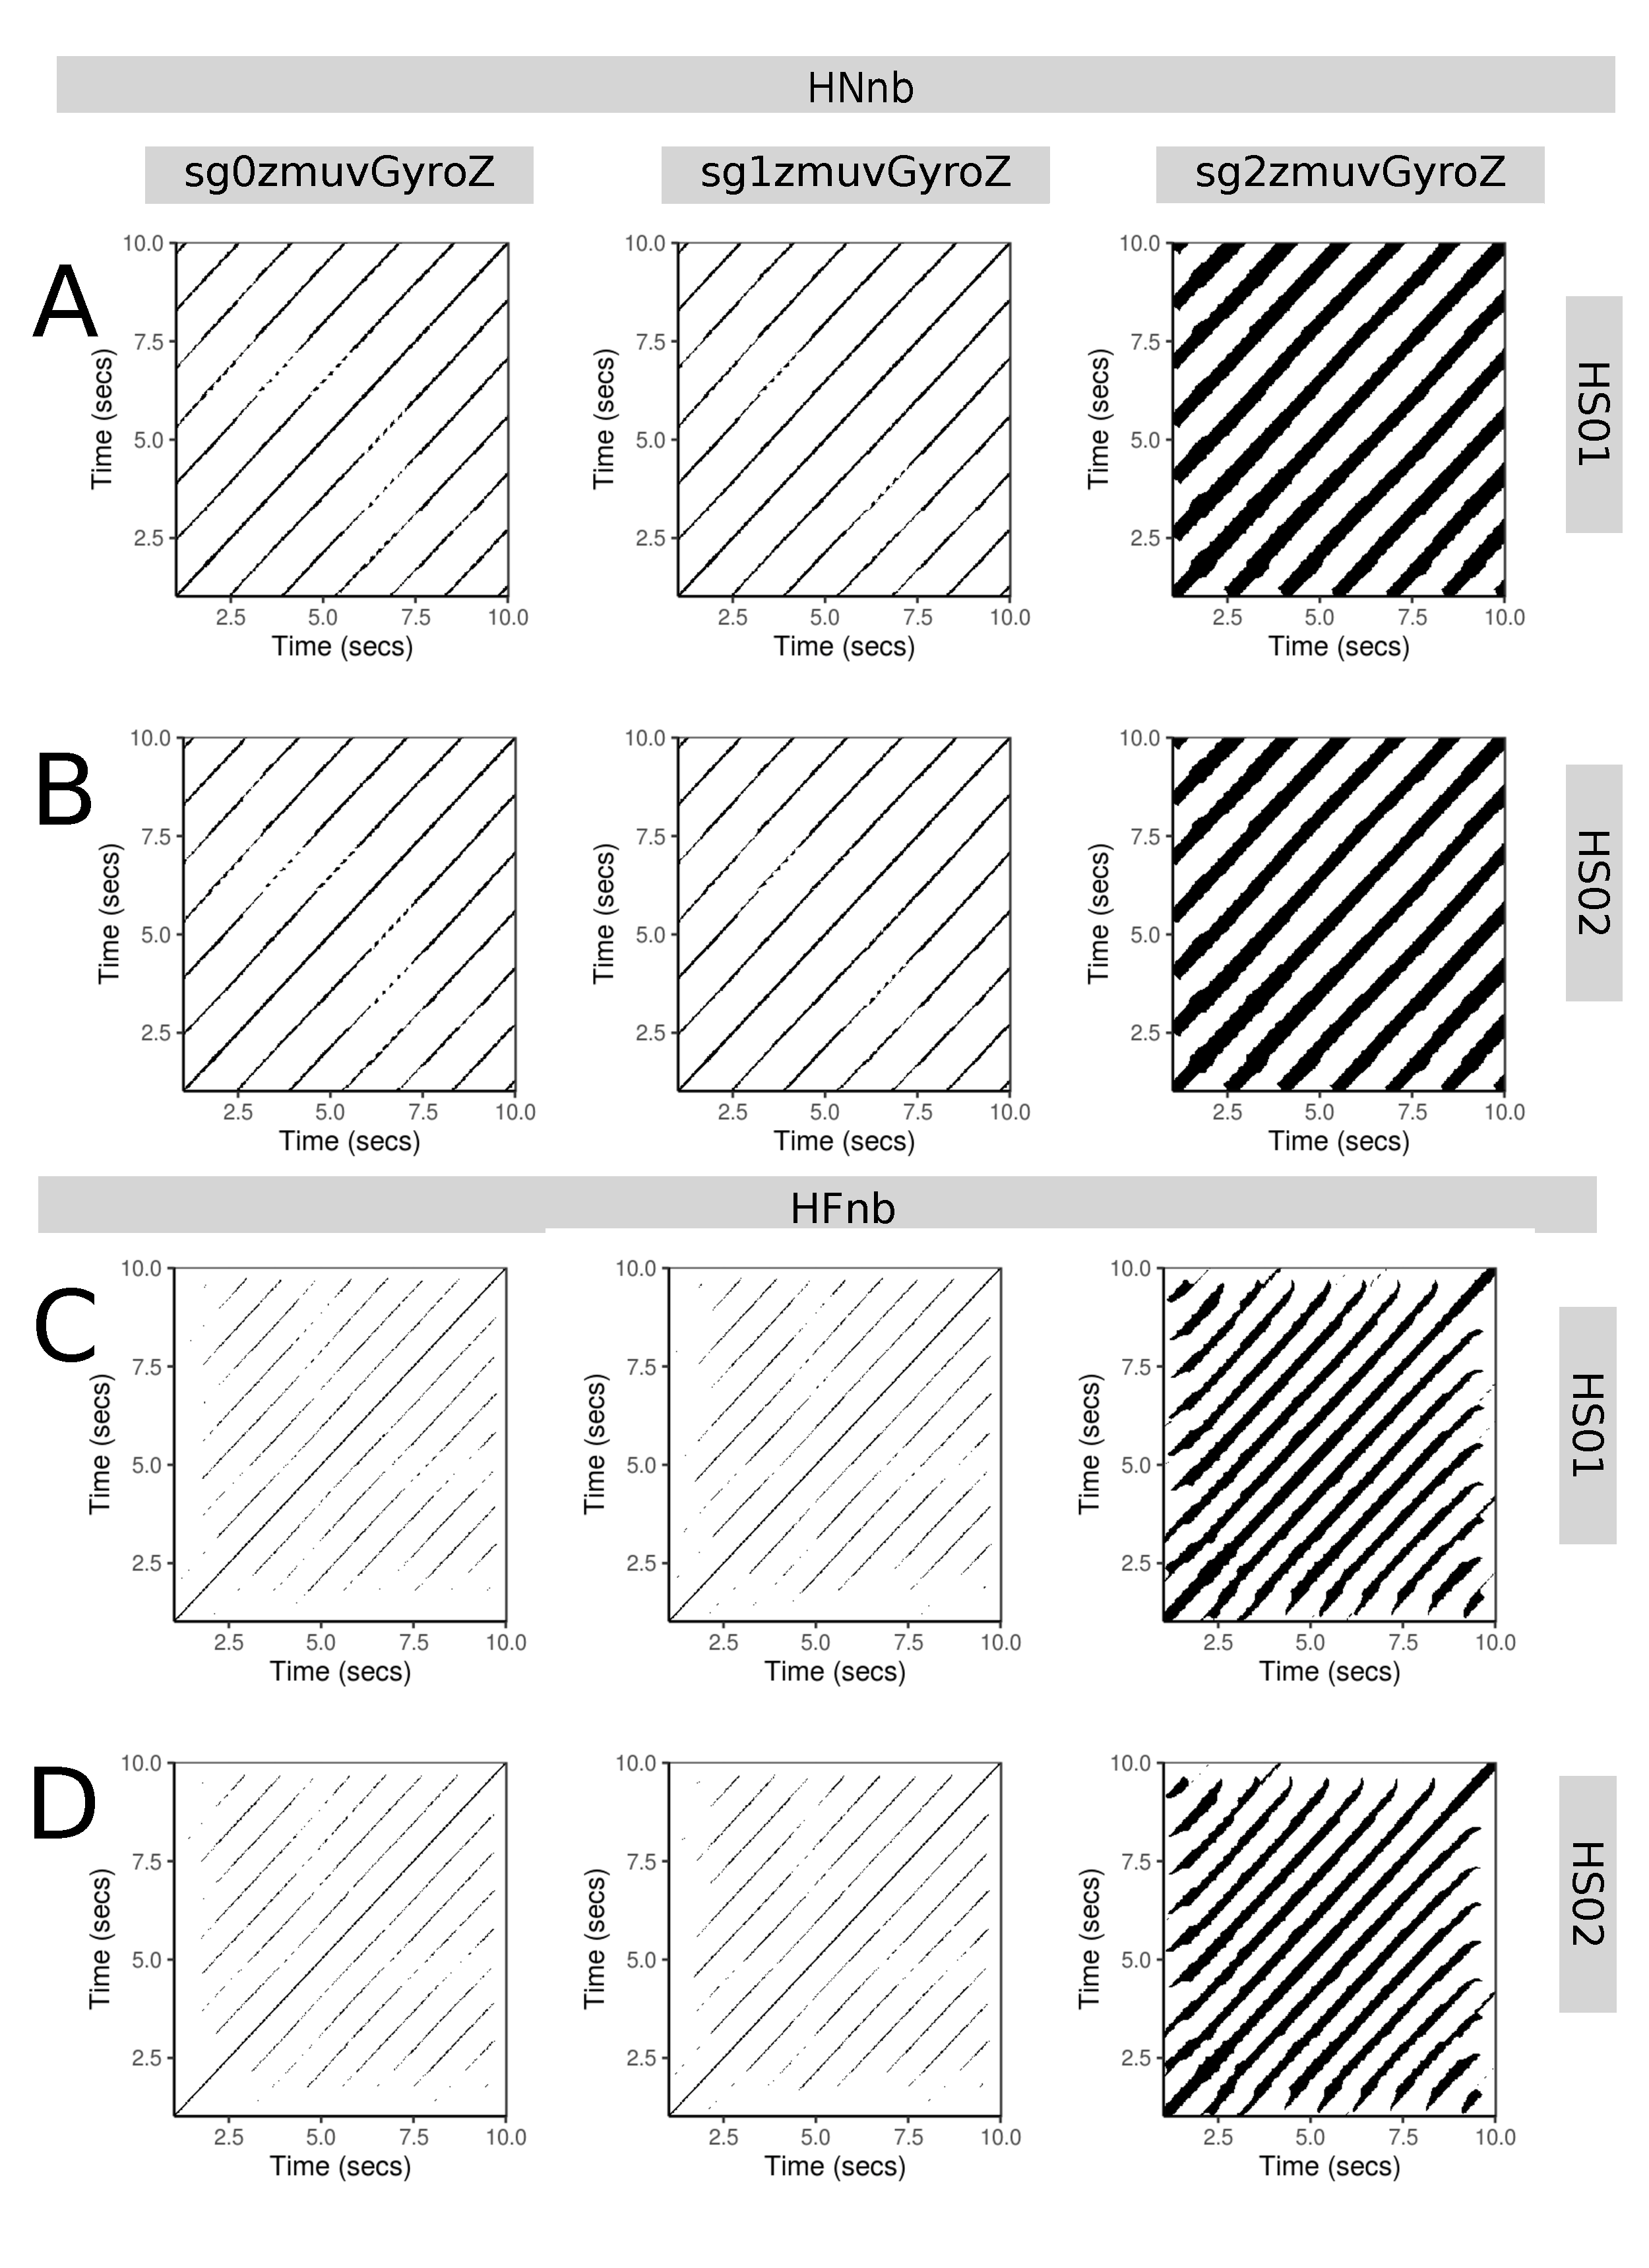
\includegraphics[height=0.8\textheight]{fig_5_09}
\caption
	[RPs for horizontal arm movements (no beat)]{
	{\bf RPs for horizontal arm movements (no beat).}	
	Recurrence plots of participant p01 for 
	(A, B) horizontal normal movements with no beat (HNnb) and
	(C, D) horizontal faster movements with no beat (HFnb).
	Time series for raw-normalised (sg0zmuvGyroZ), 
	normalised-smoothed 1 (sg1zmuvGyroZ) and 
	normalised-smoothed 2 (sg2zmuvGyroZ) with
	(A, C) sensor 01 attached to the participant (HS01), and
	(B, D) sensor 02 attached to the participant (HS02).
	Recurrence plots were computed with 
	embedding parameters $\overline{m_0}=6$, $\overline{\tau_0}=10$ and 
	recurrence threshold $\epsilon=1$.
	R code to reproduce the figure is available from \cite{xochicale2018}.
        }
    \label{fig:rps_Hnb_w500}
\end{figure}
%%---------------------------------(FIGURE)------------------------------------
%%---------------------------------(FIGURE)------------------------------------
\begin{figure}
\centering
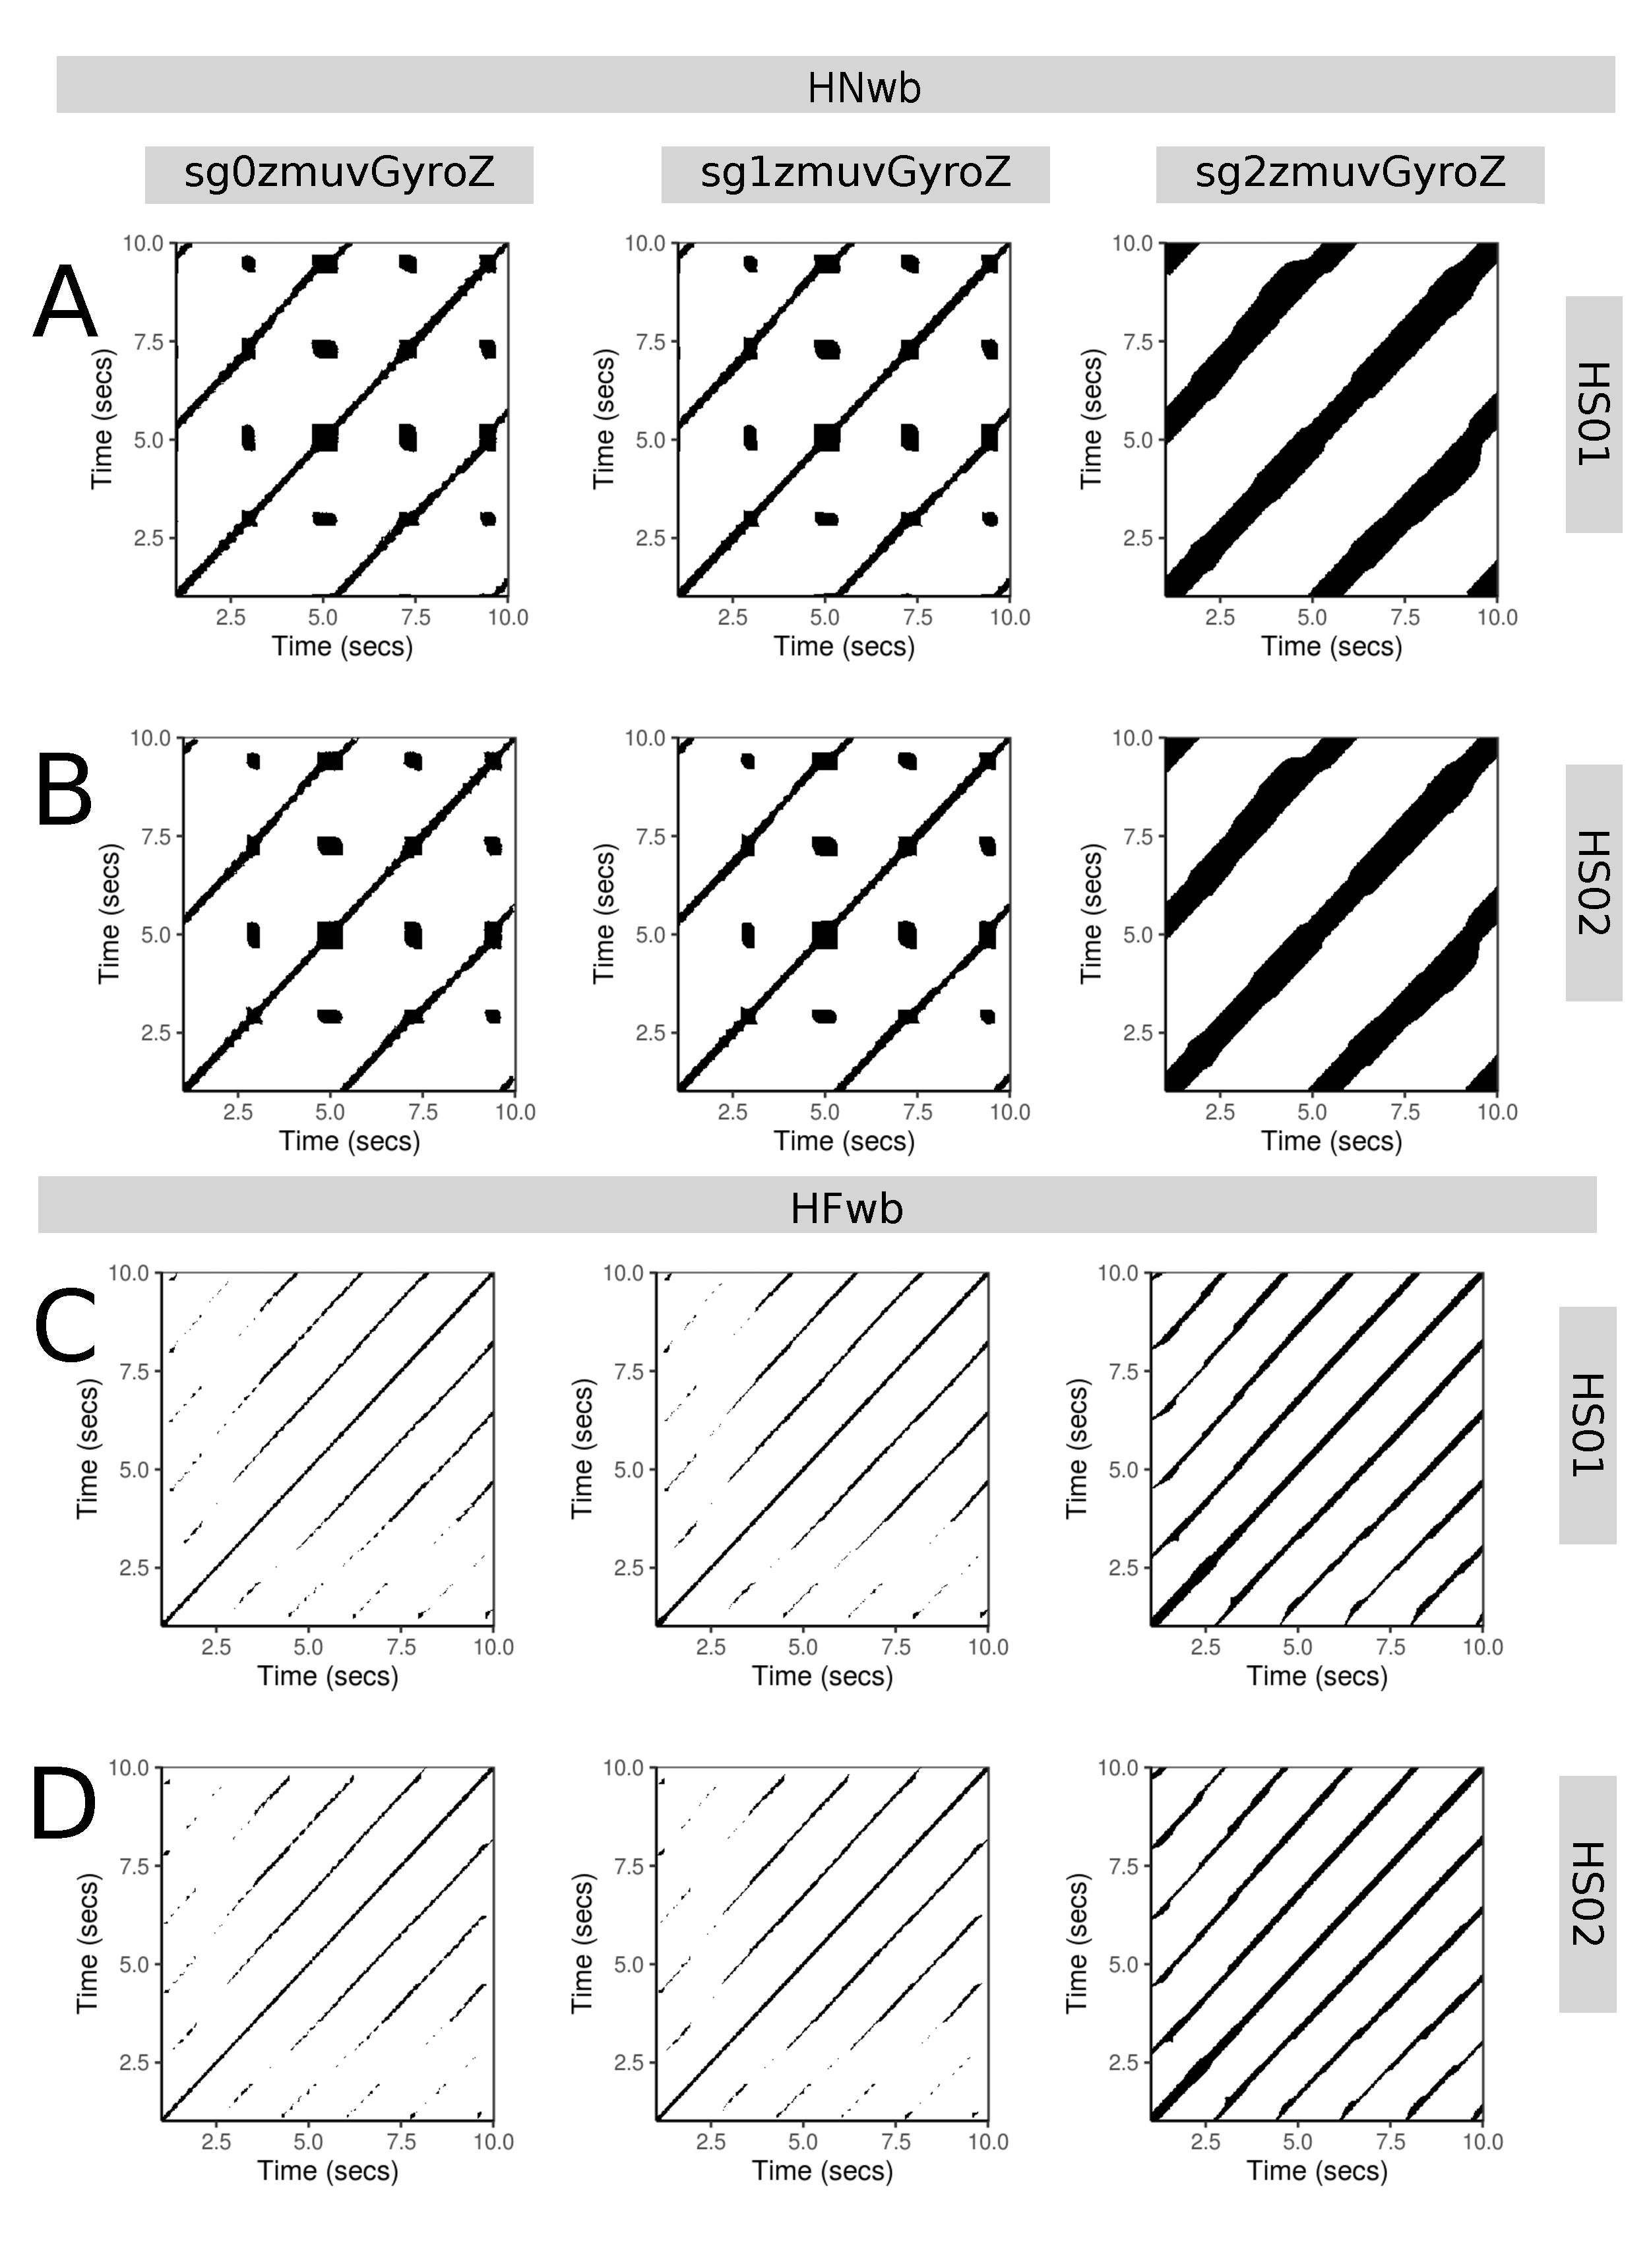
\includegraphics[height=0.8\textheight]{fig_5_10}
\caption
	[RPs for horizontal arm movements (with beat)]{
	{\bf RPs for horizontal arm movements (with beat).}	
	Recurrence plots of participant p01 for 
	(A, B) horizontal normal movements with beat (HNwb) and
	(C, D) horizontal faster movements with beat (HFwb).
	Time series for raw-normalised (sg0zmuvGyroZ), 
	normalised-smoothed 1 (sg1zmuvGyroZ) and 
	normalised-smoothed 2 (sg2zmuvGyroZ) with
	(A, C) sensor 01 attached to the participant (HS01), and
	(B, D) sensor 02 attached to the participant (HS02).
	Recurrence plots were computed with 
	embedding parameters $\overline{m_0}=6$, $\overline{\tau_0}=10$ and 
	recurrence threshold $\epsilon=1$.
	R code to reproduce the figure is available from \cite{xochicale2018}.
        }
    \label{fig:rps_Hwb_w500}
\end{figure}
%%---------------------------------(FIGURE)------------------------------------
%%---------------------------------(FIGURE)-----------------------------------
\begin{figure}
\centering
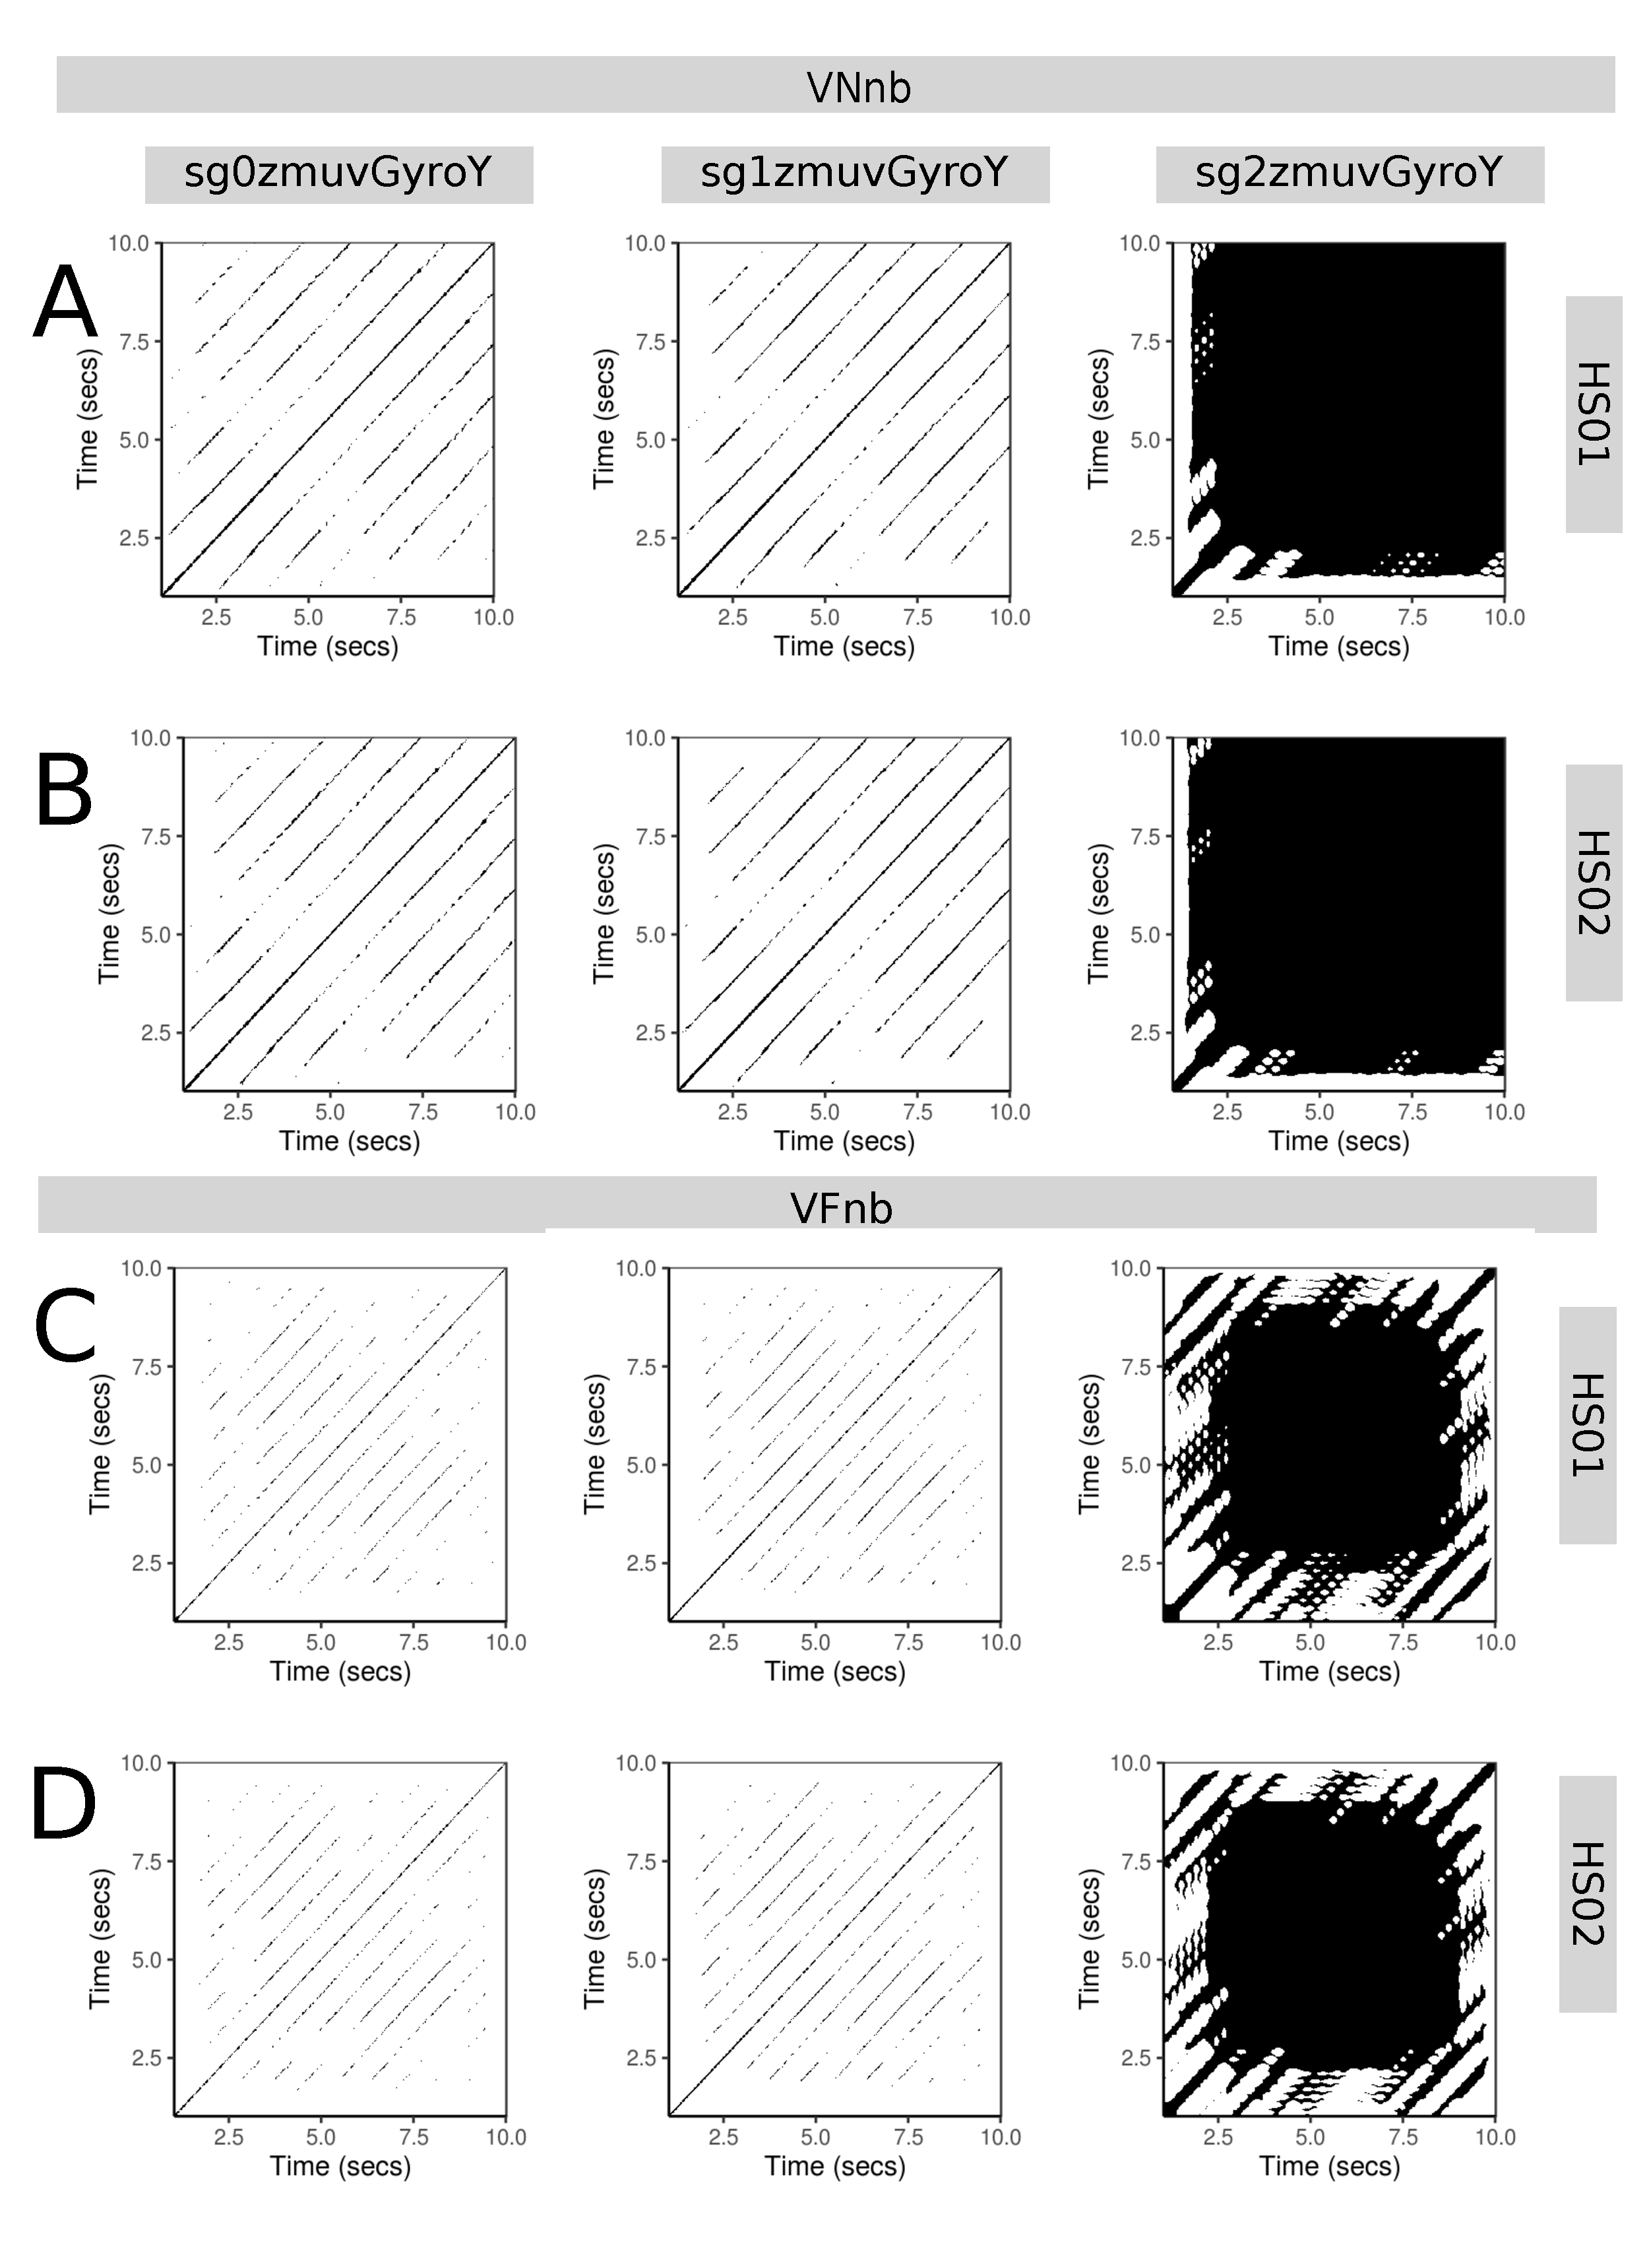
\includegraphics[height=0.8\textheight]{fig_5_11}
\caption
	[RPs for vertical arm movements (no beat)]{
	{\bf RPs for vertical arm movements (no beat).}	
	Recurrence plots of participant p01 for 
	(A, B) vertical normal movements with no beat (VNnb) and
	(C, D) vertical faster movements with no beat (VFnb).
	Time series for raw-normalised (sg0zmuvGyroY), 
	normalised-smoothed 1 (sg1zmuvGyroY) and 
	normalised-smoothed 2 (sg2zmuvGyroY) with
	(A, C) sensor 01 attached to the participant (HS01), and
	(B, D) sensor 02 attached to the participant (HS02).
	Recurrence plots were computed with 
	embedding parameters $\overline{m_0}=6$, $\overline{\tau_0}=10$ and 
	recurrence threshold $\epsilon=1$.
	R code to reproduce the figure is available from \cite{xochicale2018}.
        }
    \label{fig:rps_Vnb_w500}
\end{figure}
%%---------------------------------(FIGURE)------------------------------------
%%---------------------------------(FIGURE)-----------------------------------
\begin{figure}
\centering
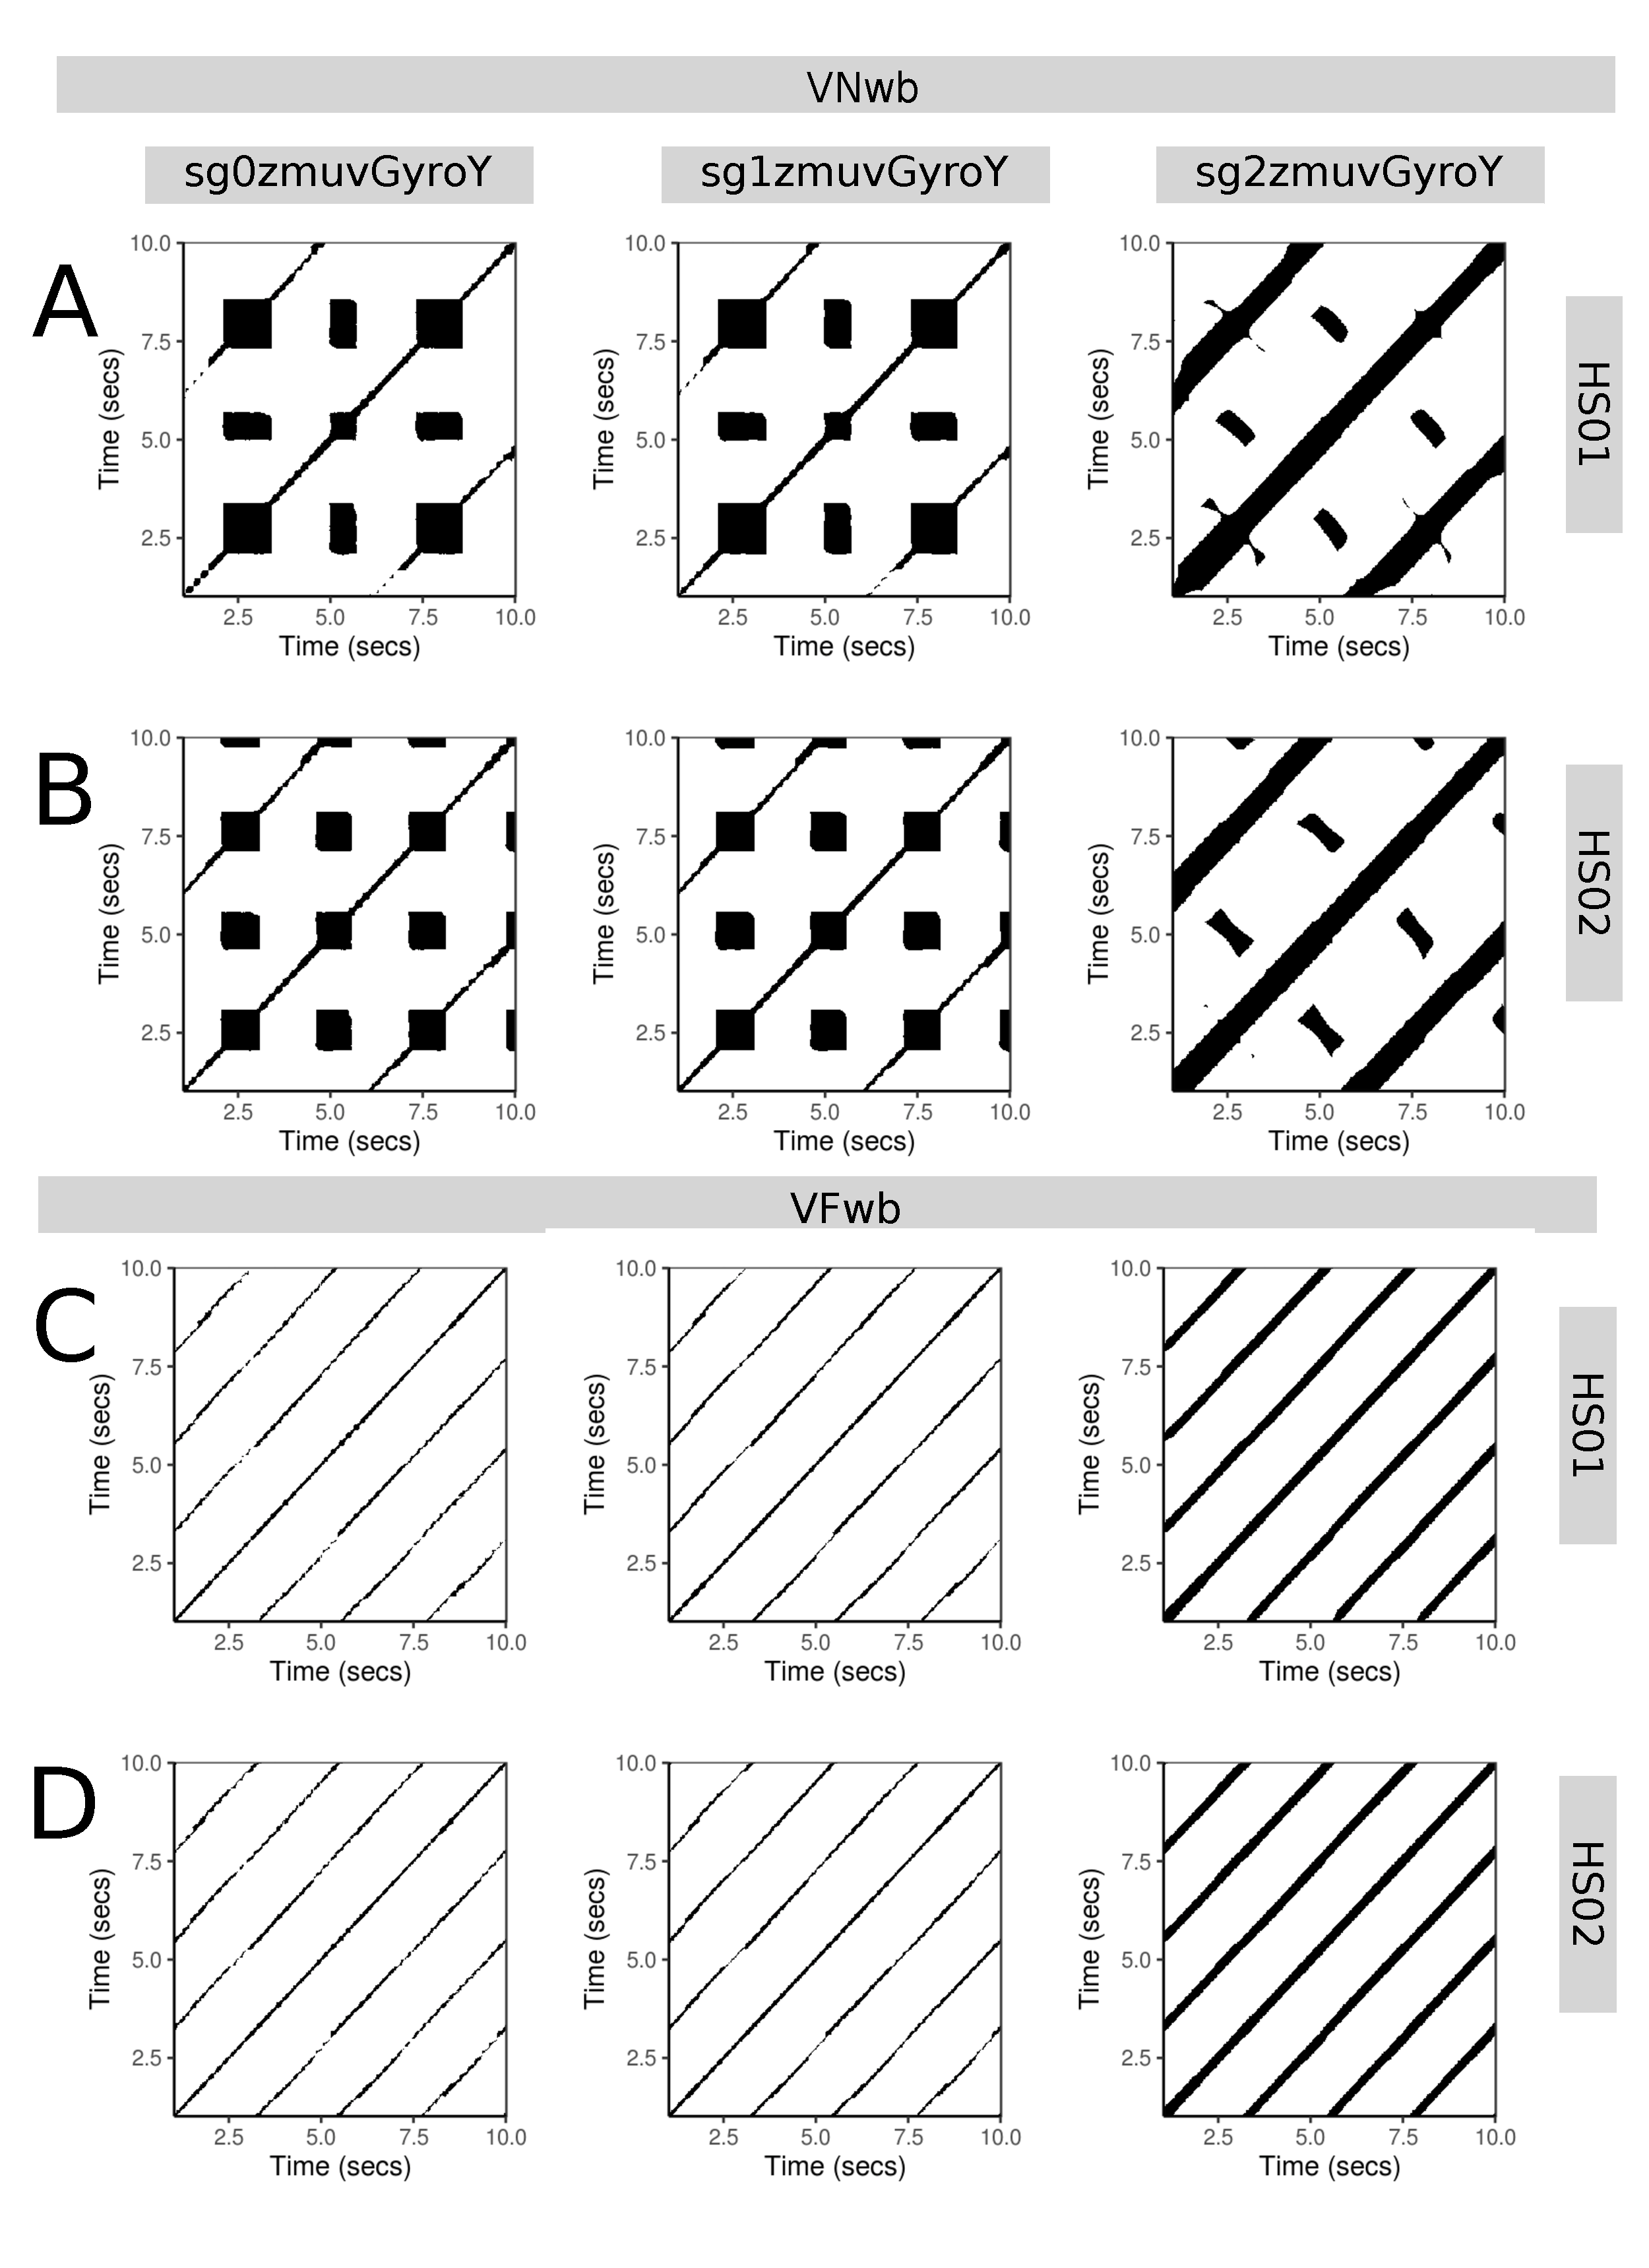
\includegraphics[height=0.8\textheight]{fig_5_12}
\caption
	[RPs for vertical arm movements (with beat)]{
	{\bf RPs for vertical arm movements (with beat).}	
	Recurrence plots of participant p01 for 
	(A, B) vertical normal movements with beat (VNwb) and
	(C, D) vertical faster movements with beat (VFwb).
	Time series for raw-normalised (sg0zmuvGyroY), 
	normalised-smoothed 1 (sg1zmuvGyroY) and 
	normalised-smoothed 2 (sg2zmuvGyroY) with
	(A, C) sensor 01 attached to the participant (HS01), and
	(B, D) sensor 02 attached to the participant (HS02).
	Recurrence plots were computed with 
	embedding parameters $\overline{m_0}=6$, $\overline{\tau_0}=10$ and 
	recurrence threshold $\epsilon=1$.
	R code to reproduce the figure is available from \cite{xochicale2018}.
        }
    \label{fig:rps_Vwb_w500}
\end{figure}
%%---------------------------------(FIGURE)------------------------------------

\newpage
\section{Recurrence Quantification Analysis} \label{ch5:rqas}
In this section is shown Recurrence Quantification Analysis (RQA) metrics 
(REC, DET, RATIO and ENTR) of six participants ($p01, p04, p05, p10, p11, p15$)
for horizontal arm movements (HNnb, HNwb, HFnb, HFwb) 
and vertical arm movements (VNnb, VNwb, VFnb, VFwb)  
with sensors HS01 and HS02, and three smoothed time series 
(sg0zmuvGyro, sg1zmuvGyro and  sg2zmuvGyro).
I hence compute four metrics of RQA metrics (REC, DET, RATIO and ENTR) with 
embedding parameters $\overline{m_0}=6$, $\overline{\tau_0}=10$ and 
recurrence threshold $\epsilon=1$.
 
\subsection*{REC values}
Figs \ref{fig:BPRQAH}(A) and \ref{fig:BPRQAV}(A) 
show box plots of REC values, representing \% of black 
dots in the RPs, for horizontal arm movements and 
vertical arm movements. 
In figs \ref{fig:BPRQAH}(A) can be noted that the interquartile range for sg2 
is greater than the sg0 and sg1 for activities HNnb and HFnb, while
REC values for activities HNwb and HFwb appear to increase 
its sample mean (gray rhombus) as the smoothness increase.
Similarly, in figs \ref{fig:BPRQAV}(A) can be seen that there is a large 
interquartile range for sg2 in activities with no beat (VNnb, VFnb), while
activities with beat (VNwb and VFwb) appear to be increase its sample
mean (gray rhombus) as the smoothness of the time series increase. 
REC values from sensors HS01 and HS01 appear to differ little 
for both horizontal and vertical arm movements. 
For further details of individual REC values of participants, see 
Figs \ref{fig:rqa_rec_H} and \ref{fig:rqa_rec_V} in 
Section \ref{appendix:d:rpas}.

\subsection*{DET values}
DET values, representing predictability and organisation of the RPs, appear
to be constant irregardless of the source of time series 
(Figs \ref{fig:BPRQAH}(B) and \ref{fig:BPRQAV}(B) ).
However, it can be noted a slight increase of DET values as the 
smoothness increase.
For further details of individual DET values of participants, see 
Figs \ref{fig:rqa_det_H}, \ref{fig:rqa_det_V} in
Section \ref{appendix:d:rpas}.

\subsection*{RATIO values}
RATIO values, representing dynamics transitions, for horizontal and 
vertical arm movements are shown in Figs 
\ref{fig:BPRQAH}(C) and \ref{fig:BPRQAV}(C).
In Figs \ref{fig:BPRQAH}(C), for vertical arm movements, 
can be noted that HNwb activity
present the less interquartile range while other seem to have similar
interquartile range. Also, the increase of smoothness makes RATIO
values to decrease (see gray rhombus).
Similarly, in Figs \ref{fig:BPRQAV}(C), for vertical arm movements, 
is shown that VNwb has the less interquartile range as well as 
sg2 for VFnb and VFwb activities. 
The increase of smoothness of time series affect in the way that 
the sample mean values of RATIO values (gray rhombus) decrease. 
For further details of individual DET values of participants, see 
Figs \ref{fig:rqa_ratio_H}, \ref{fig:rqa_ratio_V} in
Section \ref{appendix:d:rpas}.

\subsection*{ENTR values}
Figs \ref{fig:BPRQAH}(D) and \ref{fig:BPRQAV}(D) show ENTR values, 
representing the complexity of the structure of time series, 
for horizontal and vertical arm movements.
Generally, figs \ref{fig:BPRQAH}(D) and \ref{fig:BPRQAV}(D) 
illustrate that the increase of smoothness causes an increase of 
sample mean (gray rhombus) of ENTR values in each of 
the activities and sensors. 
For both vertical and horizontal ENTR values for Nwb seems 
to be a bit higher than Nnb, while Fnb and Fwb appear to be 
have similar values.
Also, there is little change between HS01 and HS02 sensors.
For further details of individual ENTR values of participants, see 
Figs \ref{fig:rqa_entr_H}, \ref{fig:rqa_entr_V} in
Section \ref{appendix:d:rpas}.

%%---------------------------------(FIGURE)-------------------------------------
\begin{figure}
\centering
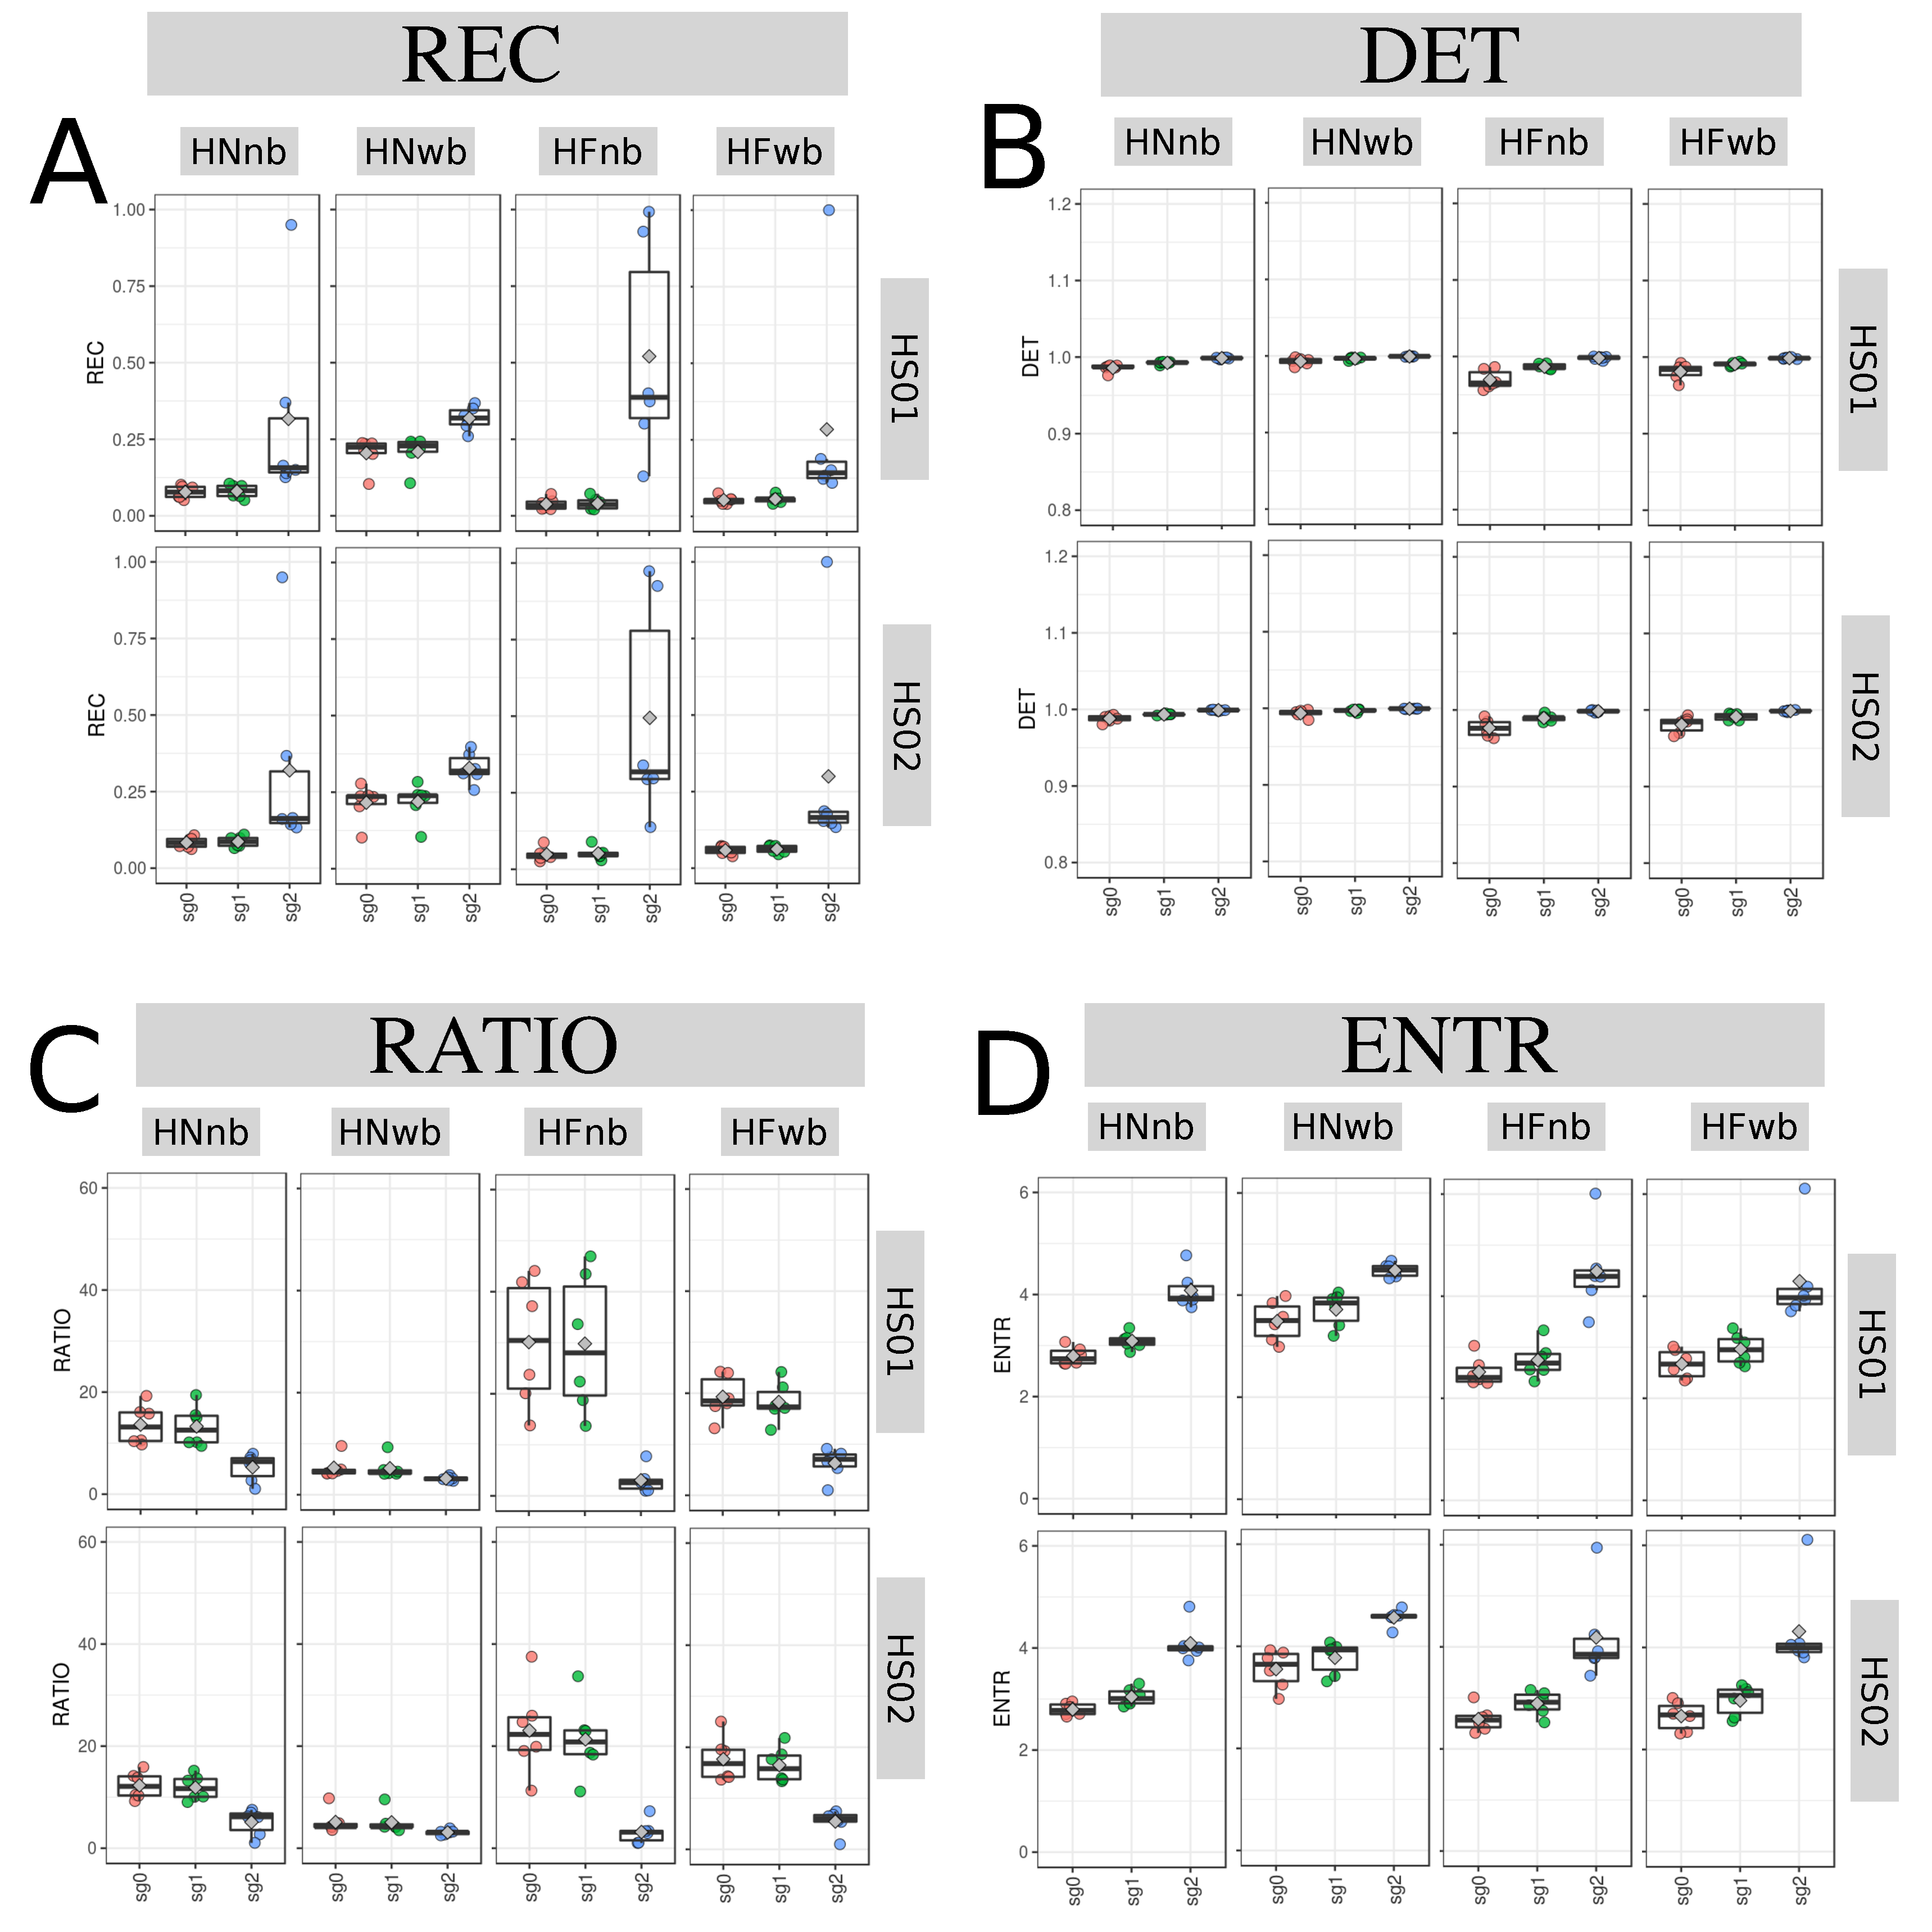
\includegraphics[width=1.0\textwidth]{fig_5_13}
	\caption
	[Box plots of RQA values for horizontal arm movements]{
	{\bf Box plots of RQA values for horizontal arm movements.}
	Box plots of (A) REC, (B) DET, (C) RATIO, and (D) ENTR values 
	for 6 participants performing HNnb, HNwb, HFnb and HFwb movements
	with sensors HS01, HS02 and three smoothed-normalised  
	time series (sg0, sg1 and sg2).
	RQA values were computed with 
	embedding parameters $\overline{m_0}=6$, $\overline{\tau_0}=10$ and 
	recurrence threshold $\epsilon=1$.
	R code to reproduce the figure is available from \cite{xochicale2018}.
        }
    \label{fig:BPRQAH}
\end{figure}
%%---------------------------------(FIGURE)-------------------------------------

%%---------------------------------(FIGURE)-------------------------------------
\begin{figure}
\centering
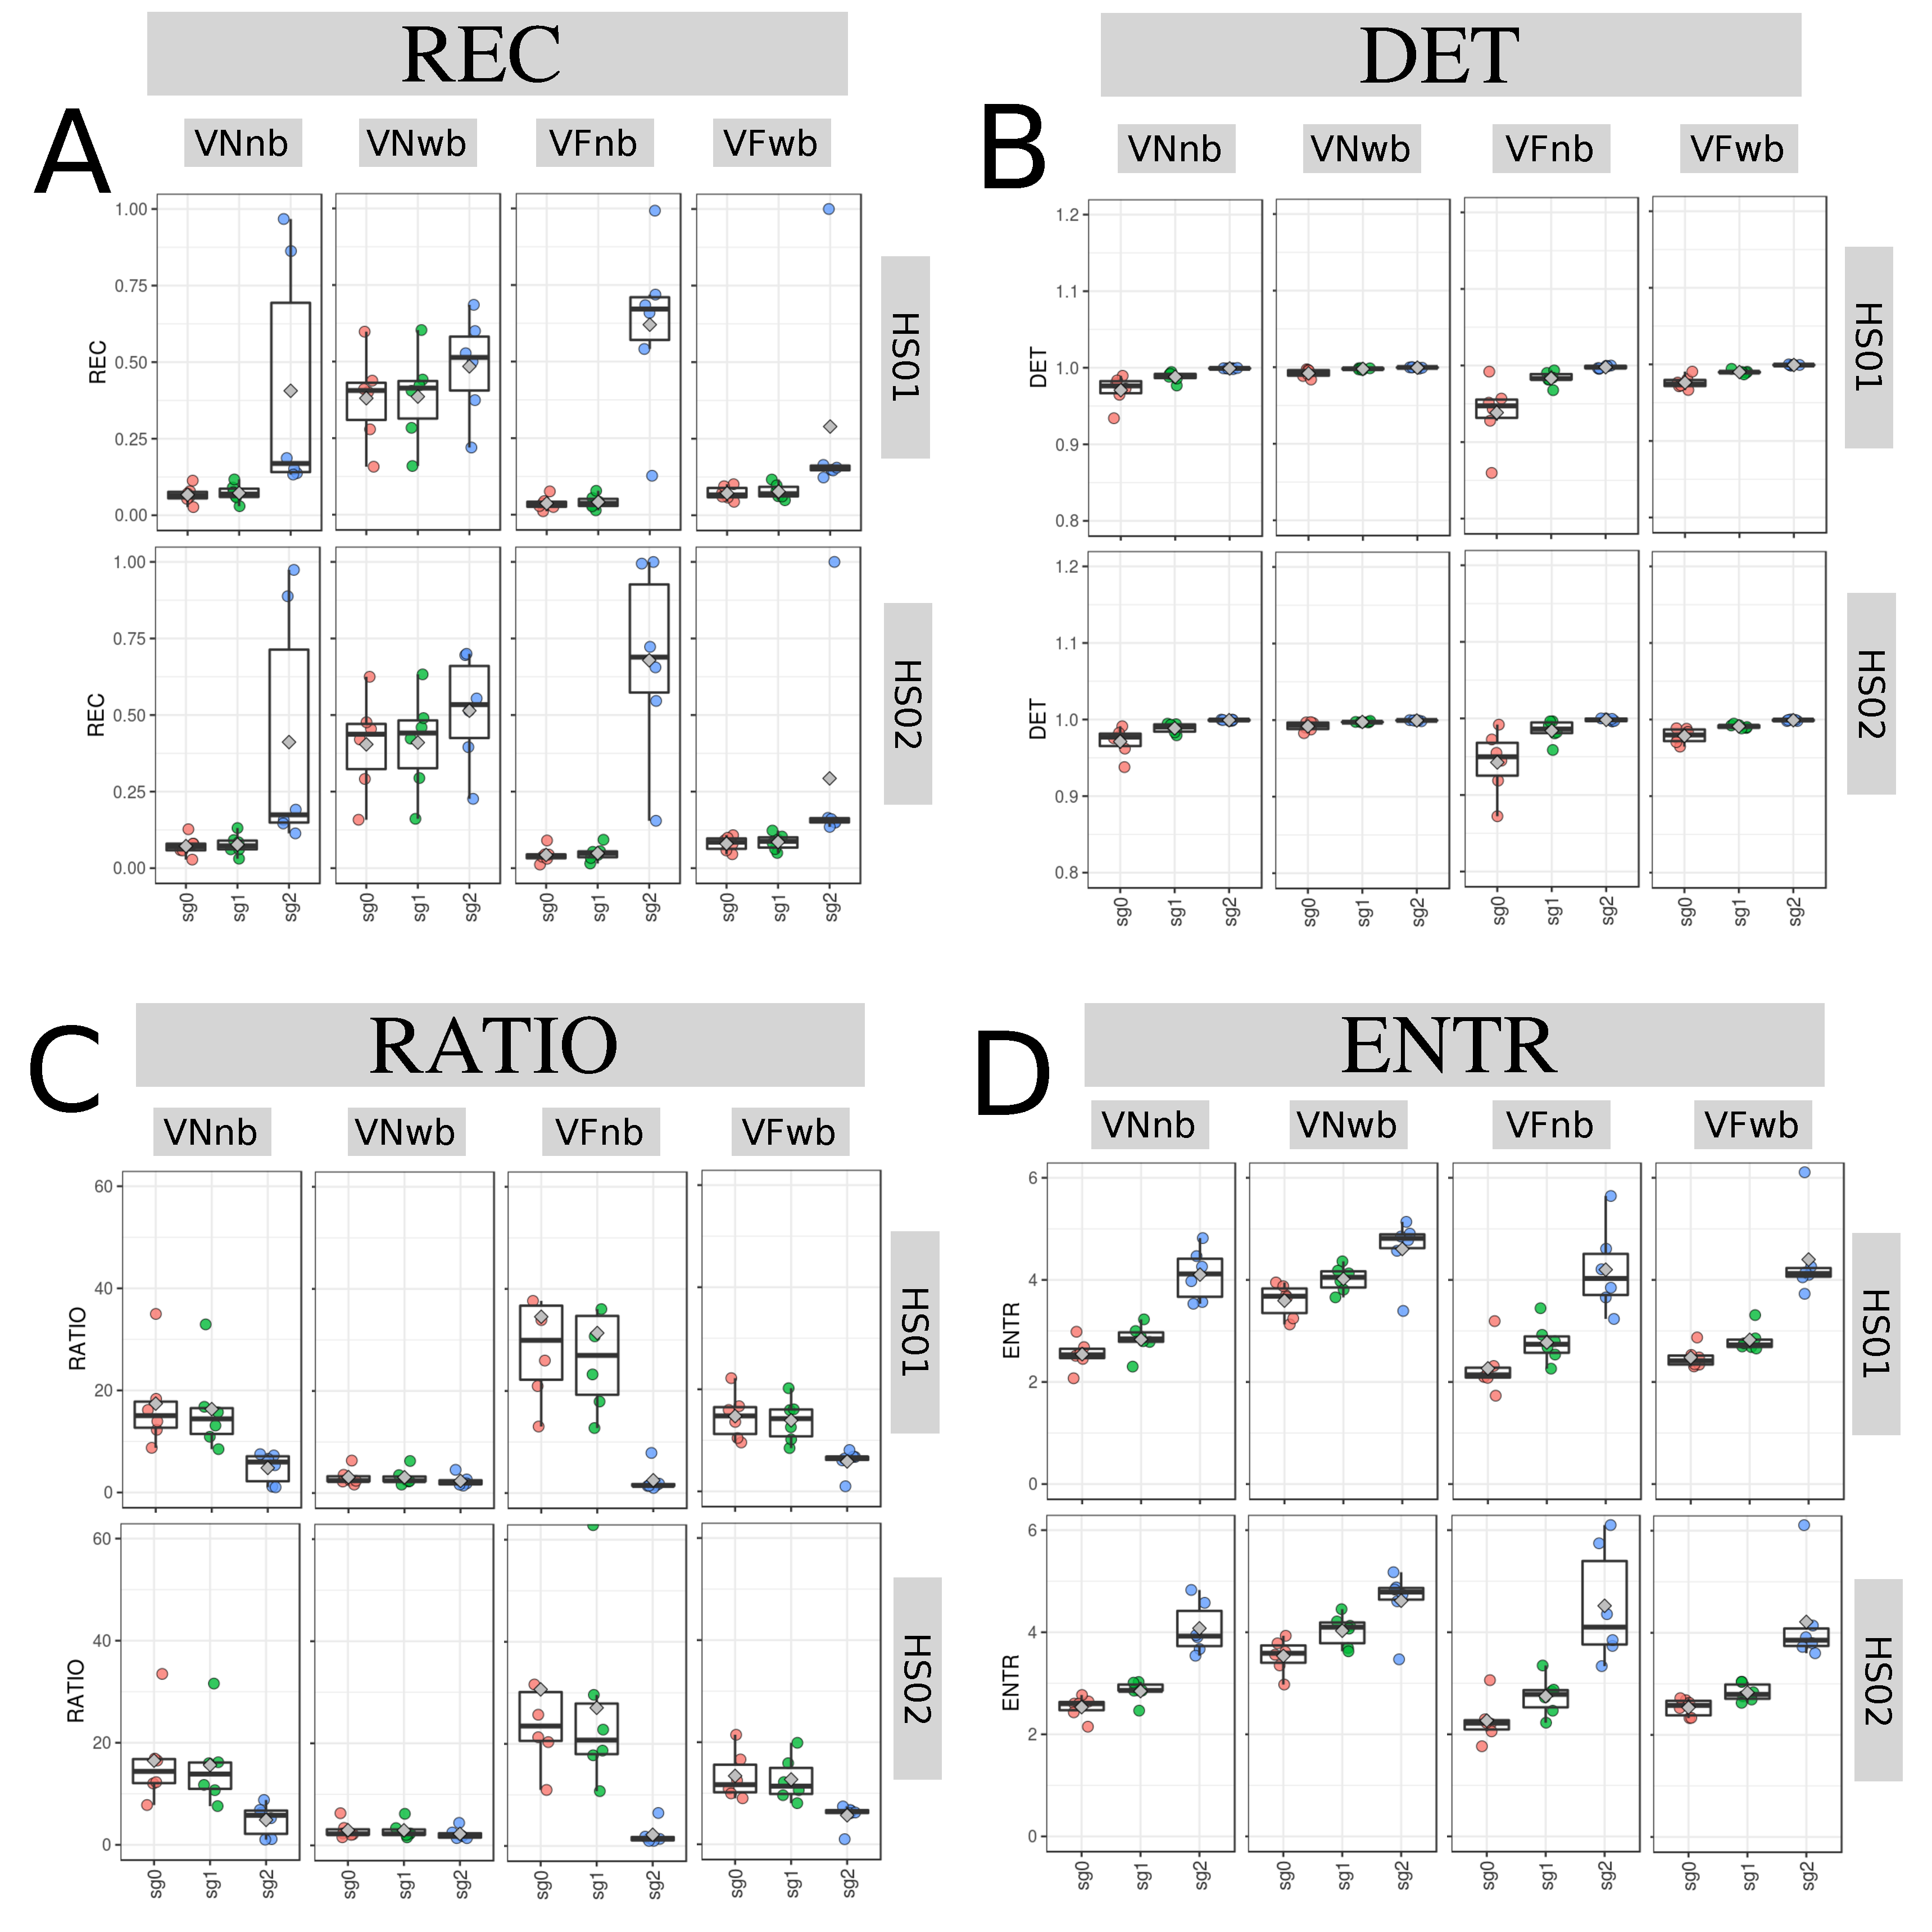
\includegraphics[width=1.0\textwidth]{fig_5_14}
	\caption
	[Box plots for RQA values for vertical arm movements]{
	{\bf Box plots for RQA values for vertical arm movements.} 
 	Box plots of (A) REC, (B) DET, (C) RATIO, and (D) ENTR values 
	for 6 participants performing VNnb, VNwb, VFnb and VFwb movements
	with sensors HS01, HS02 and three smoothed-normalised  
	time series (sg0, sg1 and sg2).
	RQA values were computed with 
	embedding parameters $\overline{m_0}=6$, $\overline{\tau_0}=10$ and 
	recurrence threshold $\epsilon=1$.
	R code to reproduce the figure is available from \cite{xochicale2018}.
        }
    \label{fig:BPRQAV}
\end{figure}
%%---------------------------------(FIGURE)-------------------------------------

\newpage
\section{Weaknesses and strengths of RQA} \label{wsRQAhii}
Surfaces for RQA metrics (REC, DET, RATIO, ENTR) are computed with the 
variation of embedding values by an increase of one 
($0 \ge m \le 10$, $0 \ge \tau \le 10$) 
and recurrence thresholds by an increase of 0.1 ($0.2 \ge \epsilon \le 3$).
Hence, we show different characteristics of 3D surfaces of RQA considering 
different activities, sensors, window size lengths and level of smoothness 
and participants.

Figs \ref{fig:topo_rqas_w500} show the surfaces for RQA metrics 
(REC, DET, RATIO, ENTR) using time series of participant $p01$, 
sensor HS01, activity HNnb, sg0zmuvGyroZ axis and a 500 window 
size length.
The 3D surface for REC values, representing the \% of recurrence dots 
in the RP, show highest values of REC when embedding values 
are near to 1 and the recurrence threshold is at the maximum 
($\epsilon = 3$ for this surfaces). Similarly, it can be seen a decrease
of REC values as the embedding dimension and embedding delay values 
increase, however there is an increase of REC values as the recurrence 
threshold is increasing (Fig \ref{fig:topo_rqas_w500}(A)).
Regarding the 3D surface for DET values, representing predictability 
and organisation of the RPs, Fig \ref{fig:topo_rqas_w500}(B) show slightly 
uniform values when varying both embedding parameters and recurrence 
threshold with the exception of embedding parameters near to 1 and 
recurrence thresholds near to 0.2 where the DET values are smaller.
3D surface for RATIO values, representing dynamic transitions, show 
a plateau with low values recurrence threshold values greater than 1.0.
However, there is a fluctuated increase of RATIO values as the embedding 
values increase given that the recurrence threshold is lower 
than 1 (Fig \ref{fig:topo_rqas_w500}(C)).
For ENTR values, representing the complexity of the structure of the 
time series, Fig \ref{fig:topo_rqas_w500}(D) show a maximum value of 
ENTR when embedding parameters are near to 1 and recurrence threshold values
are near to 3.0. It can also be noted fluctuations in the 3D surface 
when ENTR values are greater than 2.5 (red surface) for embedding 
dimensions between 3 to 9 and a decrease of ENTR values per each 
embedding dimension for delay embedding values (yellow surface).
Additionally, ENTR values decrease as the embedding dimension and 
delay embedding decrease.
%%---------------------------------(FIGURE)-----------------------------------
\begin{figure}[h!]
\centering
\includegraphics[width=1.0\textwidth]{fig_5_15}
    \caption
	[3D surface plots of RQA metrics]{
	{\bf 3D surface plots of RQA metrics.}
	3D surface plots of RQA metrics (A) REC, (B) DET, (C) RATIO and 
	(D) ENTR with an increasing pair of embedding parameters 
	($0 \le m_0 \le 10$, $0 \le \tau_0 \le 10$) 
	and recurrence thresholds ($ 0.2 \le \epsilon_r \le 3 $).
	RQA metrics are computed with the time series of participant $p01$ using 
	HS01 sensor, HNnb activity, sg0zmuvGyroZ axis and 500 samples 
	for window size length.
        R code to reproduce the figure is available from \cite{xochicale2018}.
	}
\label{fig:topo_rqas_w500}
\end{figure}
%%---------------------------------(FIGURE)------------------------------------

\newpage
\subsection{Sensors and activities}
Figs \ref{fig:topo_s_hs01_H_w500} and \ref{fig:topo_s_hs02_H_w500} show
3D surfaces of RQA metrics (REC, DET, RATIO, ENTR) for horizontal arm 
movements (HNnb, HNwb, HFnb, HFwb) using sensor HS01 and HS02 
for participant $p01$ with sg0zmuvGyroZ axis and 500 window size lenght.
Hence, Figs \ref{fig:topo_s_hs01_H_w500} present 3D surfaces of RQA metrics 
for HS01, where 3D surfaces for REC values 
(Fig \ref{fig:topo_s_hs01_H_w500}(A)) appear to be similar across 
the activities (HNnb, HFnb, HFwb) with the exception of HNwb which 
decrease of REC values is mainly affected by the increase of recurrence 
threshold and slightly affected to the increase of embedding dimension 
parameters. For DET values, 3D surfaces in Figs \ref{fig:topo_s_hs01_H_w500}(B)
appear to show values near to 1.0 (red colour surface), however HNwb 
shown fluctuations of DET values as the embedding dimension increase, 
it can also be noted a decrease of DET values for certain values of 
recurrence threshold (2.6 for HNwb, 0.3 for HFnb, and 0.3 for HFwb).
For Fig \ref{fig:topo_s_hs01_H_w500}(C)), 3D surfaces for RATIO values 
appear to be similar, showing a plateau for values between 0 to 50 
(blue surface) and the increase of peaks is different for each of the 
activities.
For Fig \ref{fig:topo_s_hs01_H_w500}(D), ENTR values present different 
surface formations, for instance, 
HNnb show fluctuated higher values of ENTR (red colour surface),
whereas for activity HNwb the ENTR values are higher (red colour surface) 
for recurrence threshold near to 3.0,
ENTR values for HFnb appear to be higher when embedding dimension is near 
to 10, while higher values for ENTR values for HFwb appear to be 
when the recurrence threshold is near to 0.2.

Then, looking and comparing visually one by one of the surfaces for sensors 
HS01 and HS02 in Figs \ref{fig:topo_s_hs01_H_w500} 
and \ref{fig:topo_s_hs02_H_w500}, one can notice little differences in the 
shape of the surfaces.
Similarly, there is little variations in the surfaces for vertical arm 
movements with the sensors HS01 and HS02 
(Figs \ref{fig:topo_s_hs01_V_w500} and \ref{fig:topo_s_hs02_V_w500}).

With regards to horizontal and vertical movements, 
3D surfaces appear to be similar for REC, DET and RATIO values
with sensor HS01
(Figs \ref{fig:topo_s_hs01_H_w500} and \ref{fig:topo_s_hs01_V_w500})
and sensor HS02
(Figs \ref{fig:topo_s_hs02_H_w500} and \ref{fig:topo_s_hs02_V_w500}), 
however 3D surfaces for ENTR values in each of the arm movements
presents distinguishable variations in the surfaces,
see Figs \ref{fig:topo_s_hs01_H_w500}(D) and \ref{fig:topo_s_hs01_V_w500}(D) 
for horizontal and vertical arm movements with sensor HS01 and
Figs \ref{fig:topo_s_hs02_H_w500}(D) and \ref{fig:topo_s_hs02_V_w500}(D) 
for horizontal and vertical arm movements with sensor HS02.

%%---------------------------------(FIGURE)------------------------------------
\begin{figure}
\centering
\includegraphics[width=1.0\textwidth]{fig_5_16}
    \caption
	[3D surface plots of RQA metrics for horizontal arm movements with HS01]{
	{\bf 3D surface plots of RQA metrics for horizontal arm movements with HS01.}
	3D surface plots for (A) REC, (B) DET, (C) RATIO and (D) ENTR values 
	with increasing pair of embedding parameters 
	($0 \le m \le 10$, $0 \le \tau \le 10$) 
	and recurrence thresholds ($ 0.2 \le \epsilon \le 3 $).
	RQA metrics are computed with the time series of participant $p01$ 
	for sensors HS01, horizontal arm movement activities 
	(HNnb, HNwb, HFnb, HFwb) and 
	sg0zmuvGyroZ axis with 500 samples window size length. 
        R code to reproduce the figure is available from \cite{xochicale2018}.
	}
\label{fig:topo_s_hs01_H_w500}
\end{figure}
%%---------------------------------(FIGURE)------------------------------------

%%---------------------------------(FIGURE)------------------------------------
\begin{figure}
\centering
\includegraphics[width=1.0\textwidth]{fig_5_17}
    \caption
	[3D surface plots of RQA metrics for horizontal arm movements with HS02]{
	{\bf 3D surface plots of RQA metrics for horizontal arm movements with HS02.}
	3D surface plots for (A) REC, (B) DET, (C) RATIO and (D) ENTR values 
	with increasing pair of embedding parameters 
	($0 \le m \le 10$, $0 \le \tau \le 10$) 
	and recurrence thresholds ($ 0.2 \le \epsilon \le 3 $).
	RQA metrics are computed with the time series of participant $p01$ 
	for sensors HS02, horizontal arm movement activities 
	(HNnb, HNwb, HFnb, HFwb) and 
	sg0zmuvGyroZ axis with 500 samples window size length. 
        R code to reproduce the figure is available from \cite{xochicale2018}.
	}
\label{fig:topo_s_hs02_H_w500}
\end{figure}
%%---------------------------------(FIGURE)------------------------------------

%%---------------------------------(FIGURE)-----------------------------------
\begin{figure}
\centering
\includegraphics[width=1.0\textwidth]{fig_5_18}
    \caption
	[3D surface plots of RQA metrics for vertical arm movements with HS01]{
	{\bf 3D surface plots of RQA metrics for vertical arm movements with HS01.}
	3D surface plots for (A) REC, (B) DET, (C) RATIO and (D) ENTR values 
	with increasing pair of embedding parameters 
	($0 \le m \le 10$, $0 \le \tau \le 10$) 
	and recurrence thresholds ($ 0.2 \le \epsilon \le 3 $).
	RQA metrics are computed with the time series of participant $p01$ 
	for sensors HS01, vertical arm movements activities 
	(VNnb, VNwb, VFnb, VFwb) and 
	sg0zmuvGyroY axis with 500 samples window size length. 
        R code to reproduce the figure is available from \cite{xochicale2018}.
	}
\label{fig:topo_s_hs01_V_w500}
\end{figure}
%%---------------------------------(FIGURE)------------------------------------


%%---------------------------------(FIGURE)------------------------------------
\begin{figure}
\centering
\includegraphics[width=1.0\textwidth]{fig_5_19}
    \caption
	[3D surface plots of RQA metrics for vertical arm movements with HS02]{
	{\bf 3D surface plots of RQA metrics for vertical arm movements with HS02.}
	3D surface plots for (A) REC, (B) DET, (C) RATIO and (D) ENTR values 
	with increasing pair of embedding parameters 
	($0 \le m \le 10$, $0 \le \tau \le 10$) 
	and recurrence thresholds ($ 0.2 \le \epsilon \le 3 $).
	RQA metrics are computed with the time series of participant $p01$ 
	for sensors HS02, vertical arm movements activities 
	(VNnb, VNwb, VFnb, VFwb) and 
	sg0zmuvGyroY axis with 500 samples window size length. 
        R code to reproduce the figure is available from \cite{xochicale2018}.
	}
\label{fig:topo_s_hs02_V_w500}
\end{figure}
%%---------------------------------(FIGURE)------------------------------------

\newpage
\subsection{Window size}
3D surfaces of REC values with a short window length (100 samples) can affect
the shape of 3D surface, however for window size of 250, 500, and 700 samples,
the 3D surfaces appear to show little changes 
(Figs \ref{fig:topo_windows_hii}(A)).
For instance, one can see 3D surfaces of DET values with a window of 100 
size length is slightly different to other surfaces but keeping the plateau
(red surface) in each of the surfaces (Figs \ref{fig:topo_windows_hii}(B)).
Similarly, the 3D surfaces of RATIO values preserve the same plateau 
(blue surface) with little variations in the surfaces as window size length 
increase (Figs \ref{fig:topo_windows_hii}(C)).
3D surfaces for ENTR values appear to have similar aspects as the 
fluctuations of the curves keeps the same values (red and yellow colours).
It can also be noted that the smoothness of 3D surfaces decrease as the 
embedding dimension parameters increase and such smoothness is also affected 
by the window length (see Figs \ref{fig:topo_windows_hii}(D)).

%---------------------------------(FIGURE)-------------------------------------
\begin{figure}
\centering
\includegraphics[width=1.0\textwidth]{fig_5_20}
    \caption
	[3D surface plots of RQA metrics for different window size lengths]{
	{\bf 3D surface plots of RQA metrics for different window size lengths.}
	3D surface plots for four window lengths (w100, w250, w500 and  w750)
	and for (A) REC, (B) DET, (C) RATIO, and (D) ENTR values
	with increasing pair of embedding parameters 
	($0 \le m \le 10$, $0 \le \tau \le 10$) 
	and recurrence thresholds ($ 0.2 \le \epsilon \le 3 $).
	RQA metrics are computed with the time series of participant $p01$ 
	using HS01 sensor, HNnb activity and sg0zmuvGyroZ axis.
	R code to reproduce the figure is available from \cite{xochicale2018}.
       }
\label{fig:topo_windows_hii}
\end{figure}
%%---------------------------------(FIGURE)------------------------------------

\subsection{Smoothness}
Figs \ref{fig:topo_smoothness_hii} show the effects of three levels of 
smothness (sg0zmuvGyroZ, sg1zmuvGyroZ and sg2zmuvGyroZ) in the RQA metrics.
Generally, 3D surfaces from sg2zmuvGyroZ are affected by the smoothness.
It can also be noted that REC values and ENTR values present a slightly 
different surfaces (see Figs \ref{fig:topo_smoothness_hii}(A, D)), 
while DET and RATIO values appear to be similar which is mainly reflected in 
the colour of the curves (see Figs \ref{fig:topo_smoothness_hii}(B, C)).
In Figs \ref{fig:topo_smoothness_hii}(A), 3D surfaces for REC values tend be 
smoothed as the smoothness of the time series increase to the point where 
the increase of recurrence threshold affects the shape of the surfaces.
Similarly, in Figs  \ref{fig:topo_smoothness_hii}(D), 
3D surface for ENTR values is affected by the smoothness of the 
time series to the point that the fluctuations in the surface does change 
drastically the shape by showing only an increase of ENTR values as
the recurrence threshold increase.

%%---------------------------------(FIGURE)------------------------------------
\begin{figure}
\centering
\includegraphics[width=0.9\textwidth]{fig_5_21}
    \caption
	[3D surface plots of RQA metrics with three levels of smoothness]{
	{\bf 3D surface plots of RQA metrics with three levels of smoothness.}
	3D surface plots for 
	three levels of smoothness (sg0zmuvGyroZ, sg1zmuvGyroZ, and sg2zmuvGyroZ) 
	and for (A) REC, (B) DET, (C) RATIO, and (D) ENTR values 
	with increasing pair of embedding parameters 
	($0 \le m \le 10$, $0 \le \tau \le 10$) 
	and recurrence thresholds ($ 0.2 \le \epsilon \le 3 $).
	RQA metrics are computed with the time series of participant $p01$ with
	HS01 sensor, HNnb activity and 500 samples window length.
	R code to reproduce the figure is available from \cite{xochicale2018}.
 }
\label{fig:topo_smoothness_hii}
\end{figure}
%%---------------------------------(FIGURE)------------------------------------

\subsection{Participants}
The shape of 3D surfaces of RQA metrics is also affected when using 
time series from different participants (Figs \ref{fig:topo_participants_hii}).
For instance, 3D surface of DET values show slightly but noticeable 
differences in the fluctuations when embedding dimension and recurrence 
threshold increase (Figs \ref{fig:topo_participants_hii}(B)) which is similar 
for ENTR values where the fluctuations of the 3D surfaces changes for each 
of the participants (Figs \ref{fig:topo_participants_hii}(D)).
However, the shape of 3D surfaces for RET values and RATIO values 
is little affected with the change of participants 
(Figs \ref{fig:topo_participants_hii}(A, C)).

%%---------------------------------(FIGURE)------------------------------------
\begin{figure}
\centering
\includegraphics[width=1.0\textwidth]{fig_5_22}
    \caption
	[3D surface plots of RQA metrics with three participants]{
	{\bf 3D surface plots of RQA metrics with three participants.}
	3D surface plots for participants $p01$, $p04$ and $p05$ 
	and for (A) REC, (B) DET, (C) RATIO, and (D) ENTR 
	with increasing pair of embedding parameters 
	($0 \le m \le 10$, $0 \le \tau \le 10$) 
	and recurrence thresholds ($ 0.2 \le \epsilon \le 3 $).
	RQA metrics are computed with the time series of
	sg0zmuvGyroZ axis, HS01 sensor, HNnb activity and 500 
	samples window length.
	R code to reproduce the figure is available from \cite{xochicale2018}.
 }
\label{fig:topo_participants_hii}
\end{figure}
%%---------------------------------(FIGURE)-------------------------------------

%\newpage
\subsection{Final remarks}
Having different sources of time series (participants, sensors, 
activities, window size length or level of smoothness) produce different
results in nonlinear analyses tools (FNN, AMI, RSSs with UTDE, RPs and
RQAs) and these results can also be sensitive to perform nonlinear analysis 
with different parameters (minimum dimension threshold, 
embedding parameters or recurrence thresholds).
Hence, we created 3D surfaces of RQA metrics with the 
variation of embedding parameters and recurrence thresholds,
such surfaces appear to be helpful to understand the dynamics 
of any kind of time series with little parametrization of nonlinear tools.
For instance, 
3D surfaces of ENTR values, with only the selection of variation of range 
of parameters, show clearly differences in the shape of 3D surfaces 
irregardless of the source of the time series. Hence making 3D surfaces 
of ENTR values a robust metric which helps us to understand the dynamics 
of human movement variability from different time series data.

